% !TEX root = ../thesis.tex
%
\chapter{Results and Evaluation}
\label{sec:evaluation}

In this section, we will present and interpret the results of our experiments as presented in chapter~\ref{sec:experiments}.
This involves firstly a brief analysis of the results of the original STAMP benchmark to establish them as a baseline to legitimize or discuss the results of our Rust-based STM implementation of the algorithm as we will use the latter to evaluate Ohua's performance.\todo{Klingt bisschen als würde ich STM vs STM und dann das gegen Ohua vergleichen -> Umformulieren?}
Subsequently, we will analyze the results of our Ohua benchmarks in detail to see, whether it could be used as a suiting replacement for STM in terms of performance.

\section{Reference Measurement Results}

\begin{figure}
    \centering
    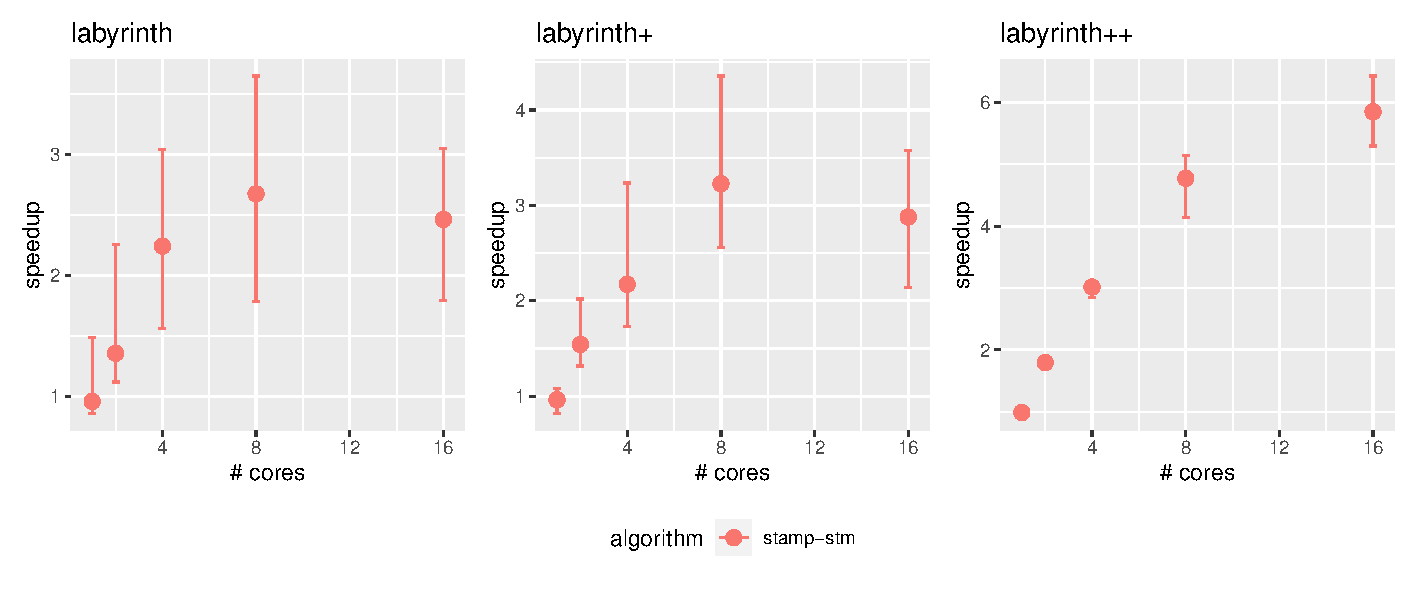
\includegraphics[width=\textwidth,keepaspectratio]{gfx/results/stamp/stamp_labyrinth_comb}
    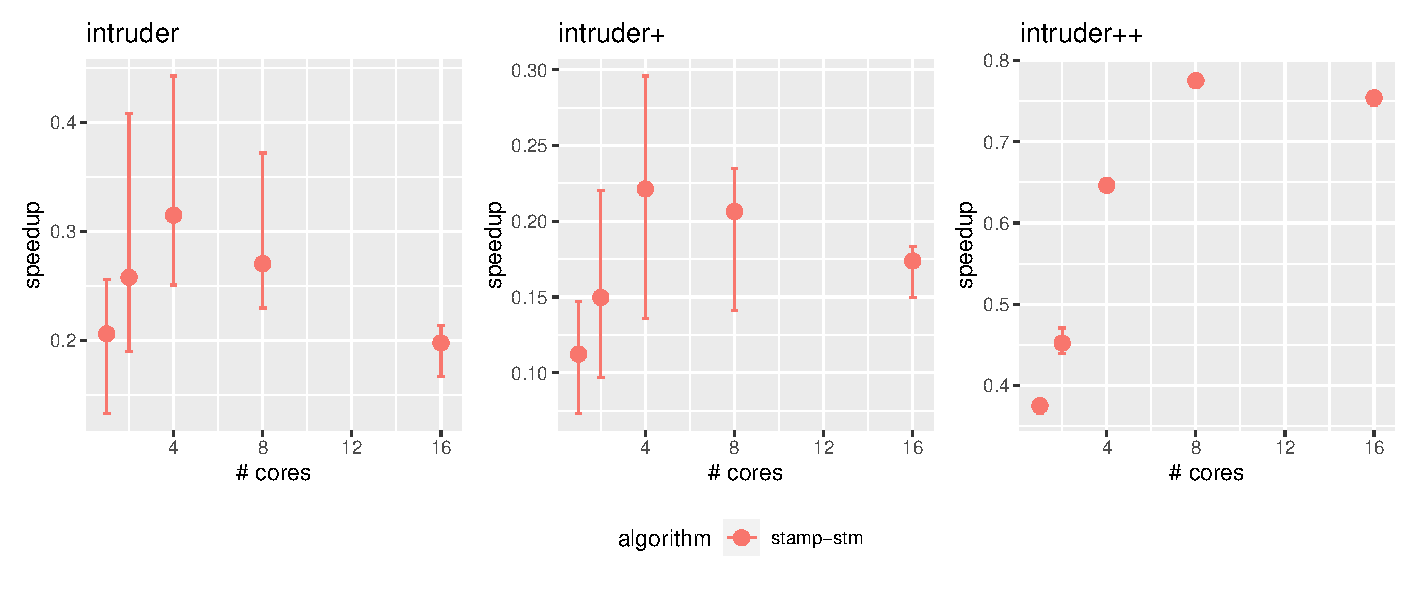
\includegraphics[width=\textwidth,keepaspectratio]{gfx/results/stamp/stamp_intruder_comb}
    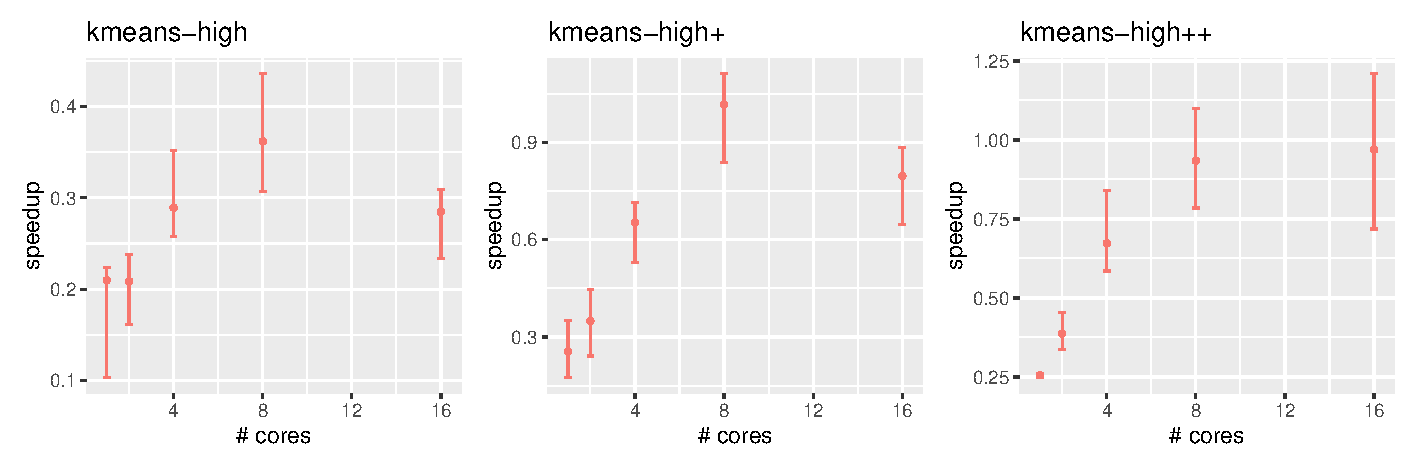
\includegraphics[width=\textwidth,keepaspectratio]{gfx/results/stamp/stamp_kmeans-high_comb}
    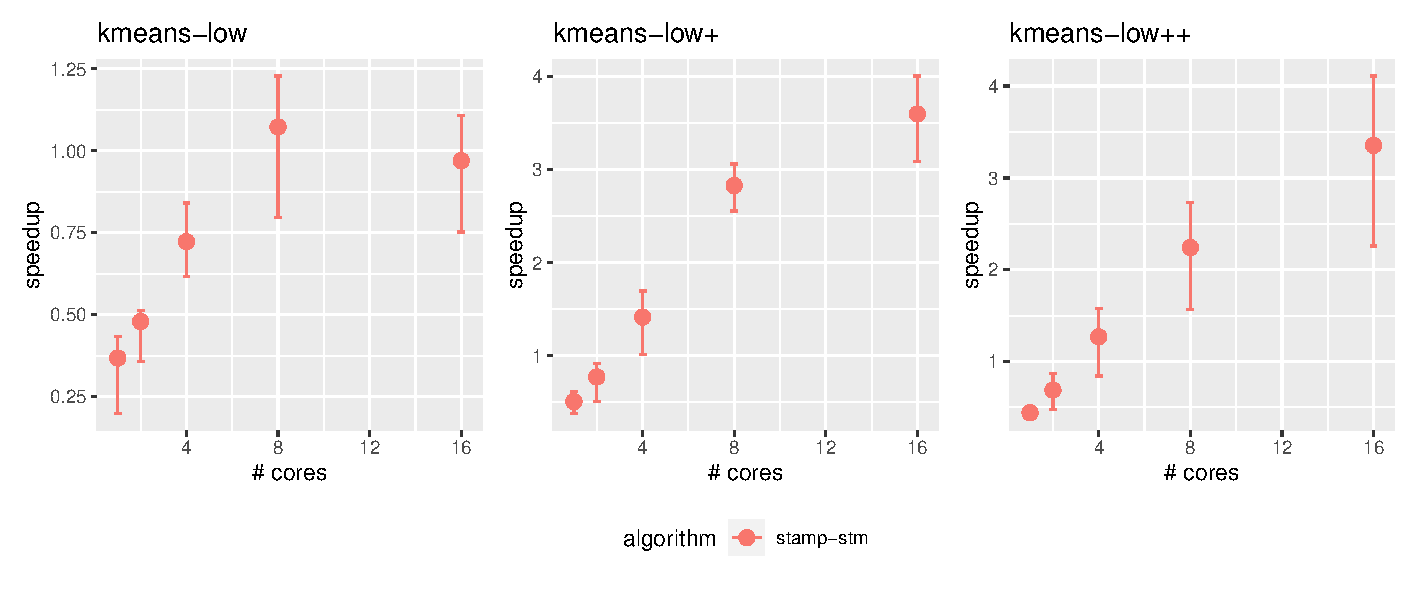
\includegraphics[width=\textwidth,keepaspectratio]{gfx/results/stamp/stamp_kmeans-low_comb}
    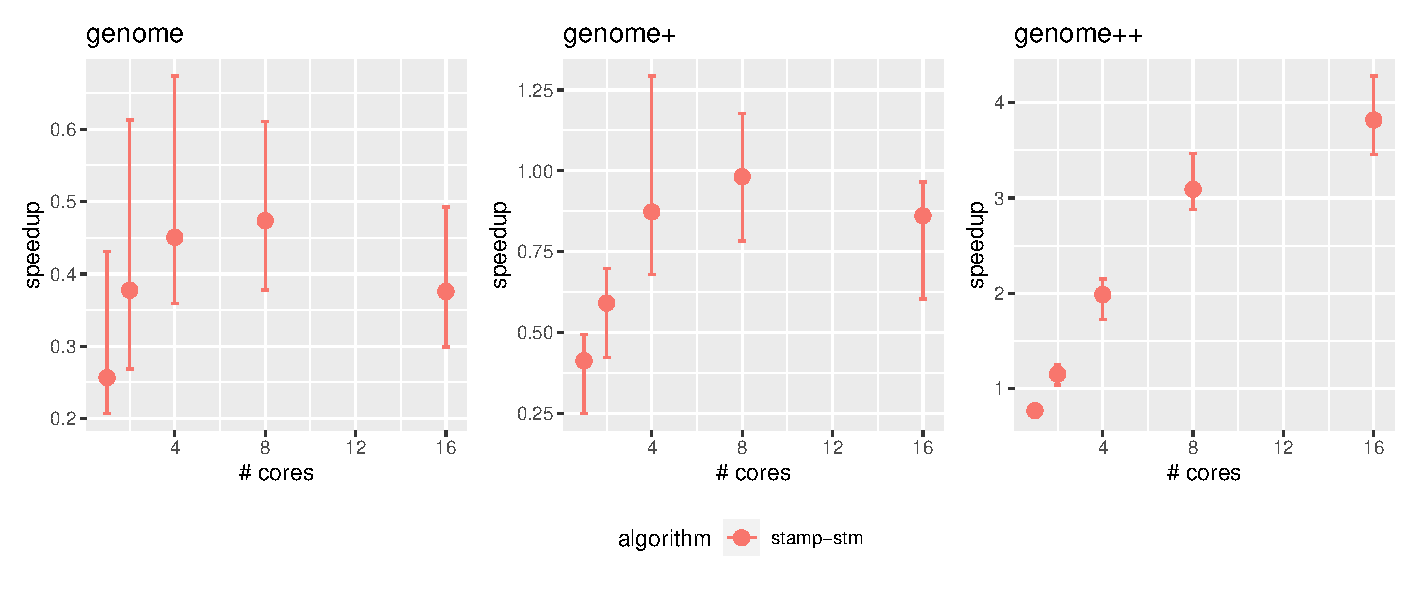
\includegraphics[width=\textwidth,keepaspectratio]{gfx/results/stamp/stamp_genome_comb}
    \caption{Speedup achieved by STM in the original STAMP  benchmarks.}%
    \label{fig:evaluation:stamp:genome}
\end{figure}

\section{Rust-based Benchmark Results}

\begin{figure}
    \centering
    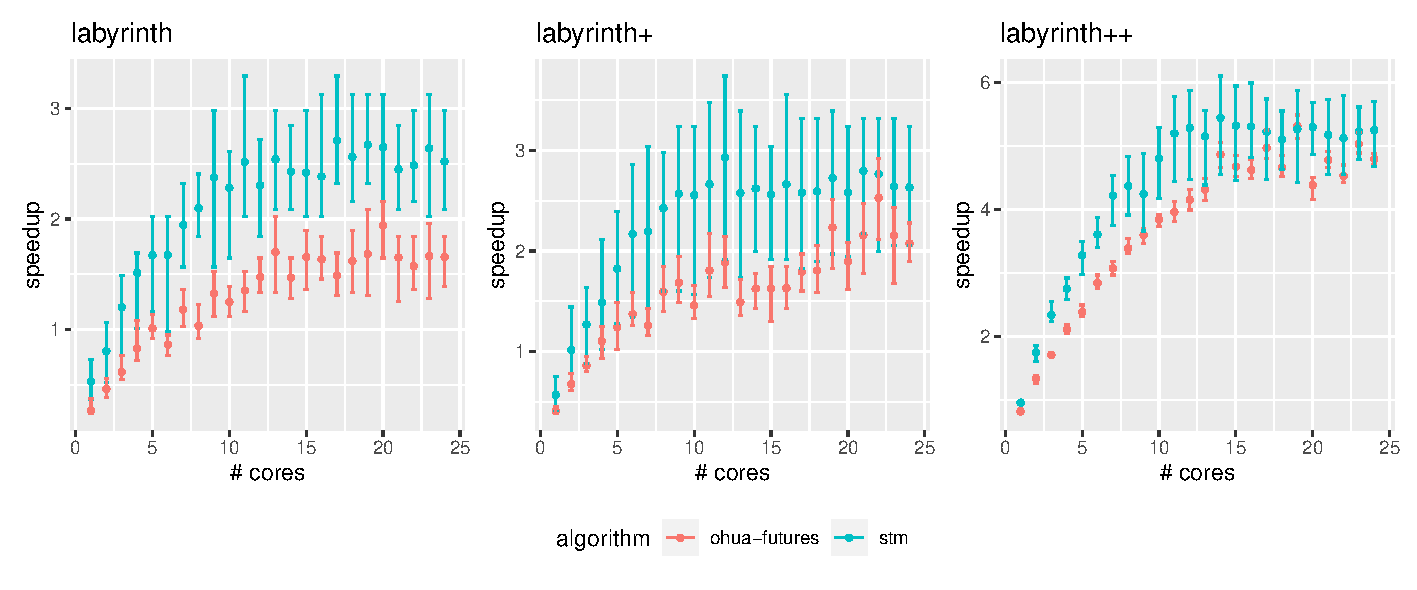
\includegraphics[width=\textwidth,keepaspectratio]{gfx/results/labyrinth_comb}
    \caption{Speedup in the labyrinth application relative to a sequential implementation.}%
    \label{fig:evaluation:labyrinth}
\end{figure}

\begin{figure}
    \centering
    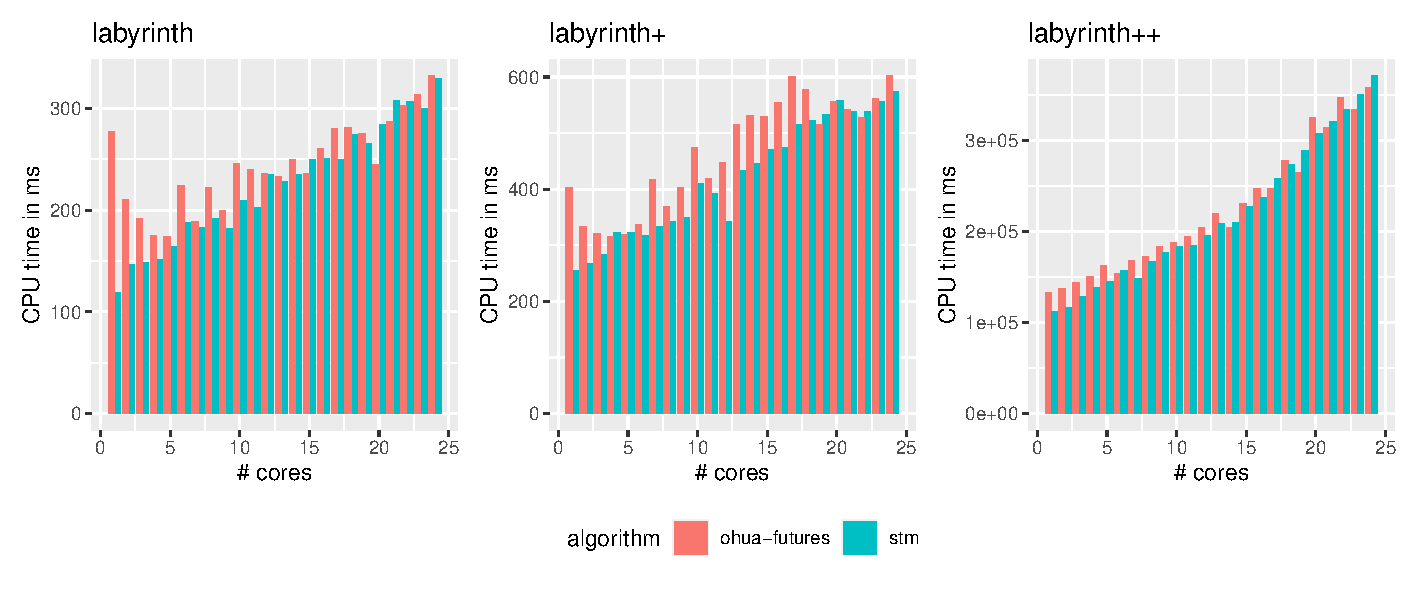
\includegraphics[width=\textwidth,keepaspectratio]{gfx/results/cpu_labyrinth_comb}
    \caption{CPU time used by both frameworks in the labyrinth application.}%
    \label{fig:evaluation:labyrinth-cpu}
\end{figure}

\begin{figure}
    \centering
    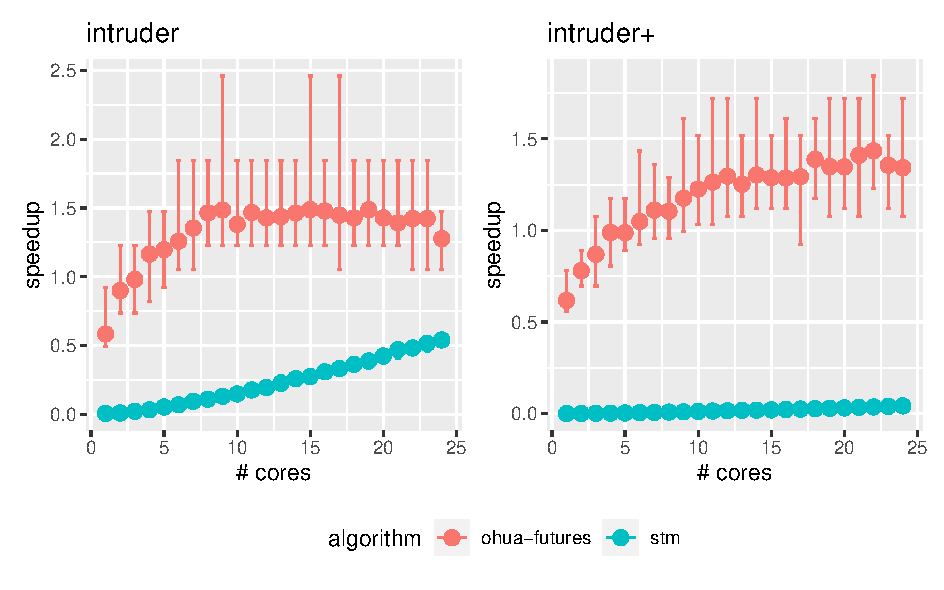
\includegraphics[width=.66\textwidth,keepaspectratio]{gfx/results/intruder_comb}
    \caption{Speedup in the intruder application relative to a sequential implementation.}%
    \label{fig:evaluation:intruder}
\end{figure}

\begin{figure}
    \centering
    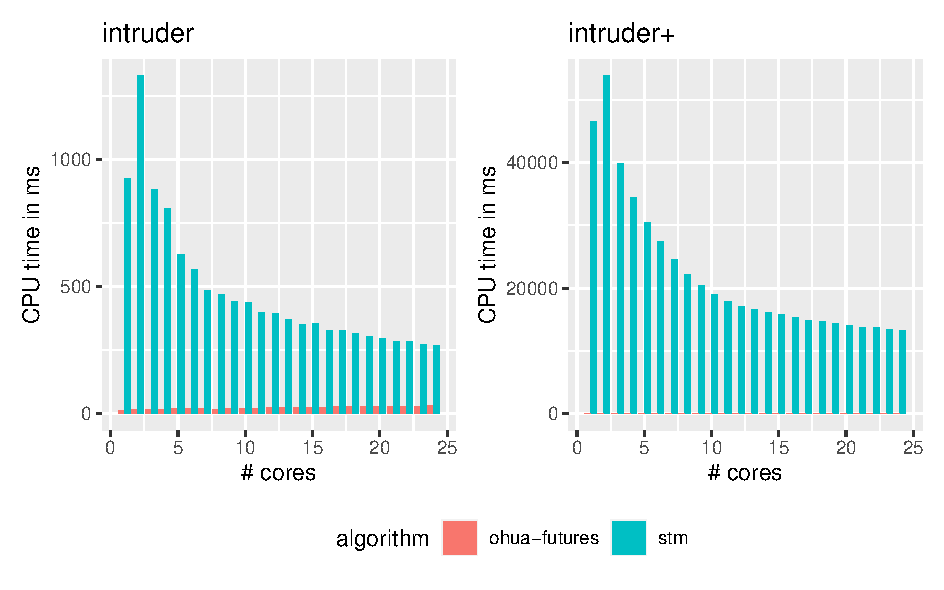
\includegraphics[width=.66\textwidth,keepaspectratio]{gfx/results/cpu_intruder_comb}
    \caption{CPU time used by both frameworks in the intruder application.}%
    \label{fig:evaluation:intruder-cpu}
\end{figure}

\begin{figure}
    \centering
    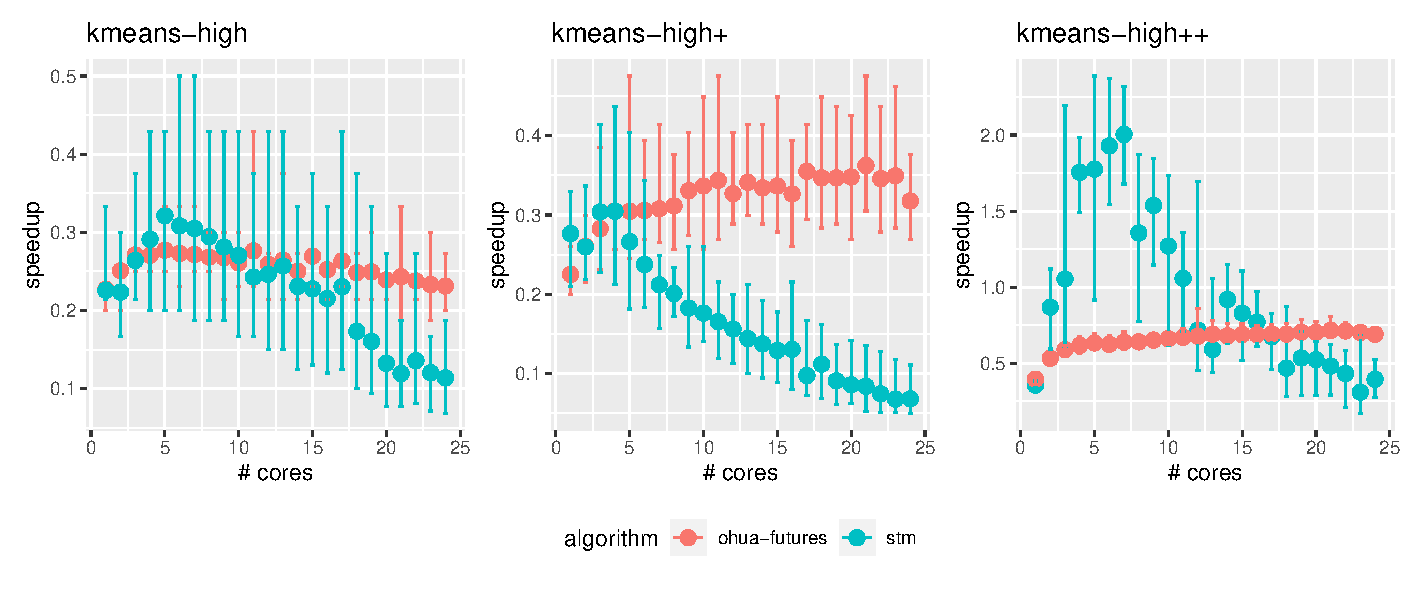
\includegraphics[width=\textwidth,keepaspectratio]{gfx/results/kmeans-high_comb}
    \caption{Speedup in the kmeans-high application relative to a sequential implementation.}%
    \label{fig:evaluation:kmeans-high}
\end{figure}

\begin{figure}
    \centering
    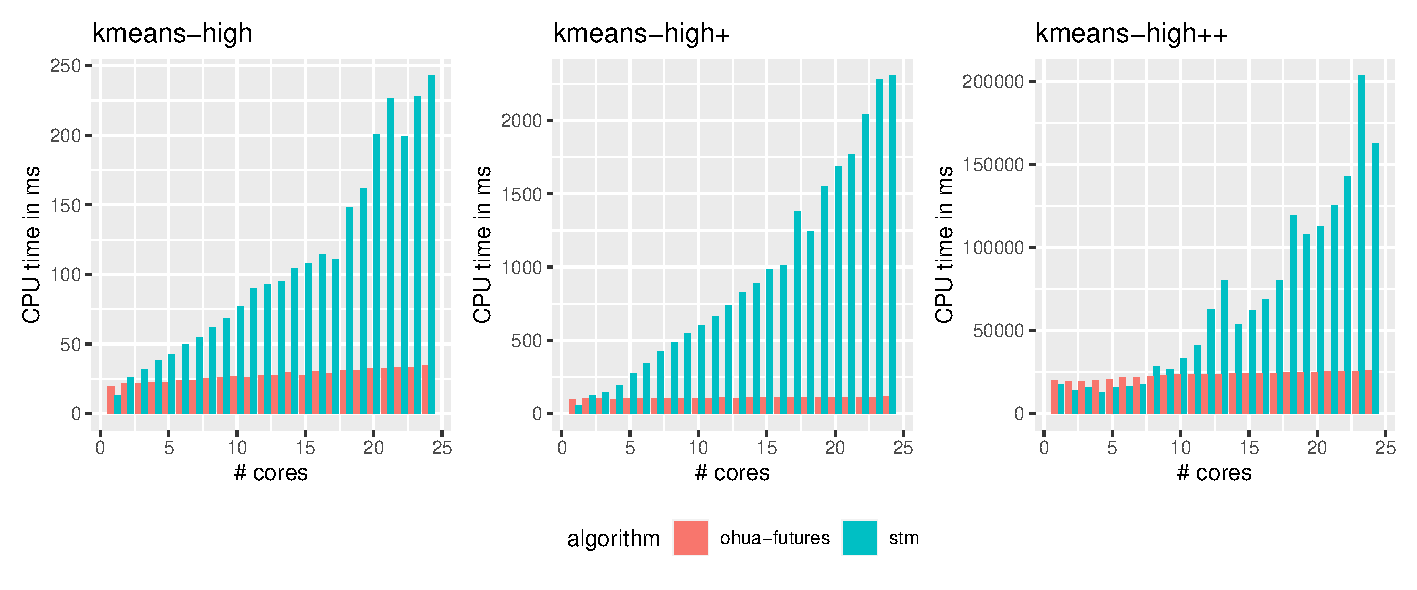
\includegraphics[width=\textwidth,keepaspectratio]{gfx/results/cpu_kmeans-high_comb}
    \caption{CPU time used by both frameworks in the kmeans-high application.}%
    \label{fig:evaluation:kmeans-high-cpu}
\end{figure}

\begin{figure}
    \centering
    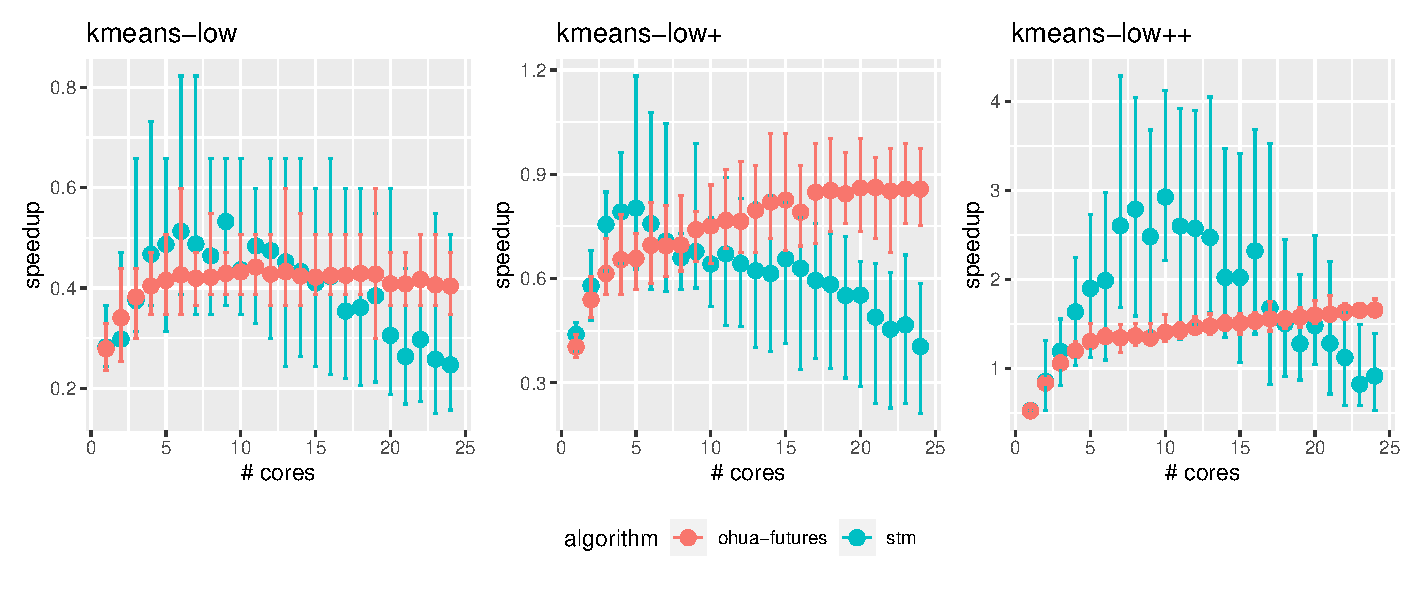
\includegraphics[width=\textwidth,keepaspectratio]{gfx/results/kmeans-low_comb}
    \caption{Speedup in the kmeans-low application relative to a sequential implementation.}%
    \label{fig:evaluation:kmeans-low}
\end{figure}

\begin{figure}
    \centering
    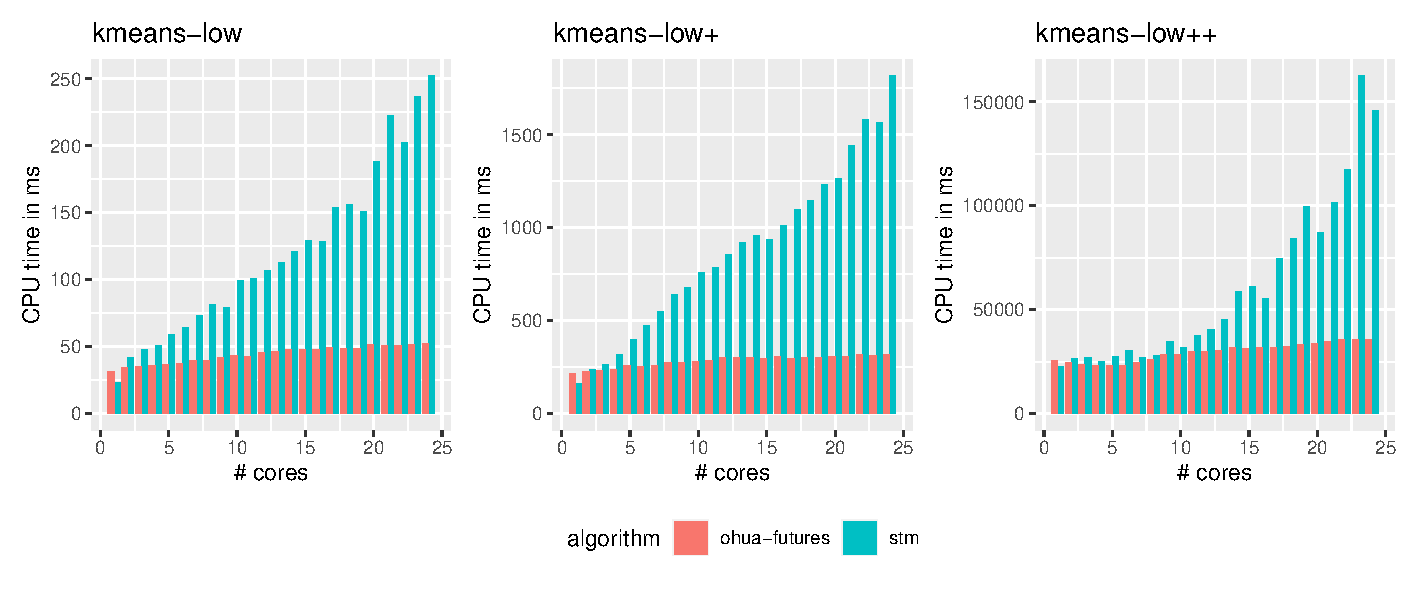
\includegraphics[width=\textwidth,keepaspectratio]{gfx/results/cpu_kmeans-low_comb}
    \caption{CPU time used by both frameworks in the kmeans-low application.}%
    \label{fig:evaluation:kmeans-low-cpu}
\end{figure}

\begin{figure}
    \centering
    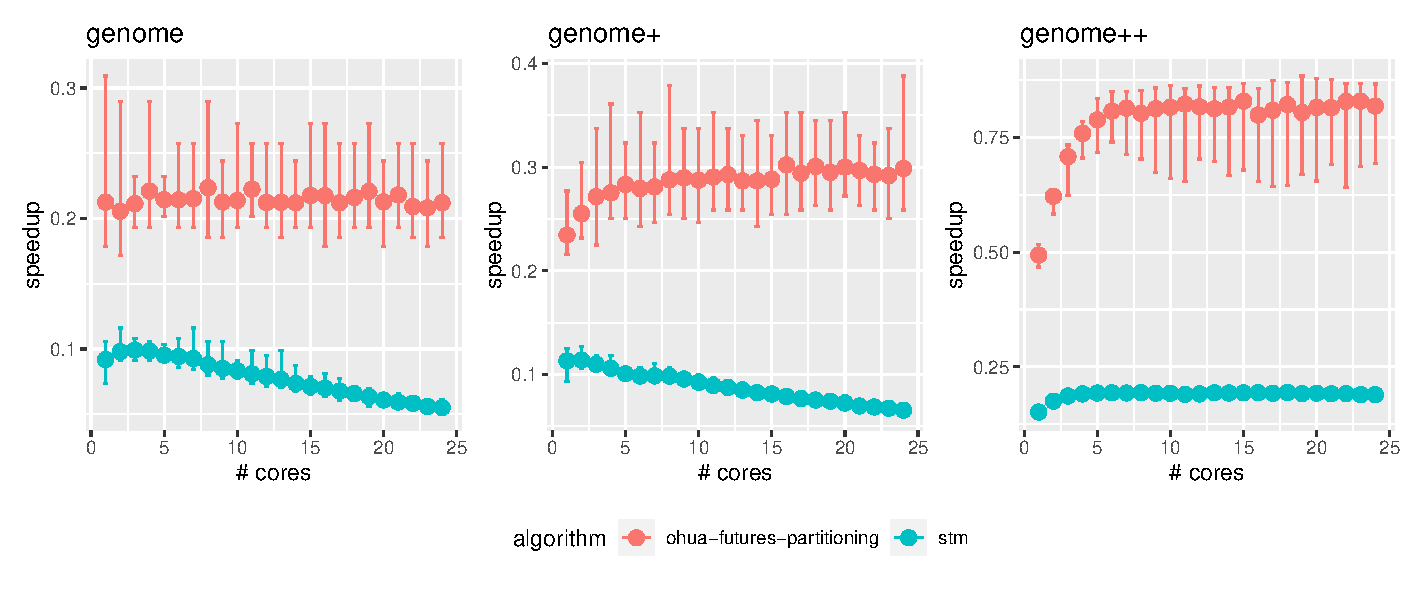
\includegraphics[width=\textwidth,keepaspectratio]{gfx/results/genome_comb}
    \caption{Speedup in the genome application relative to a sequential implementation.}%
    \label{fig:evaluation:genome}
\end{figure}

\begin{figure}
    \centering
    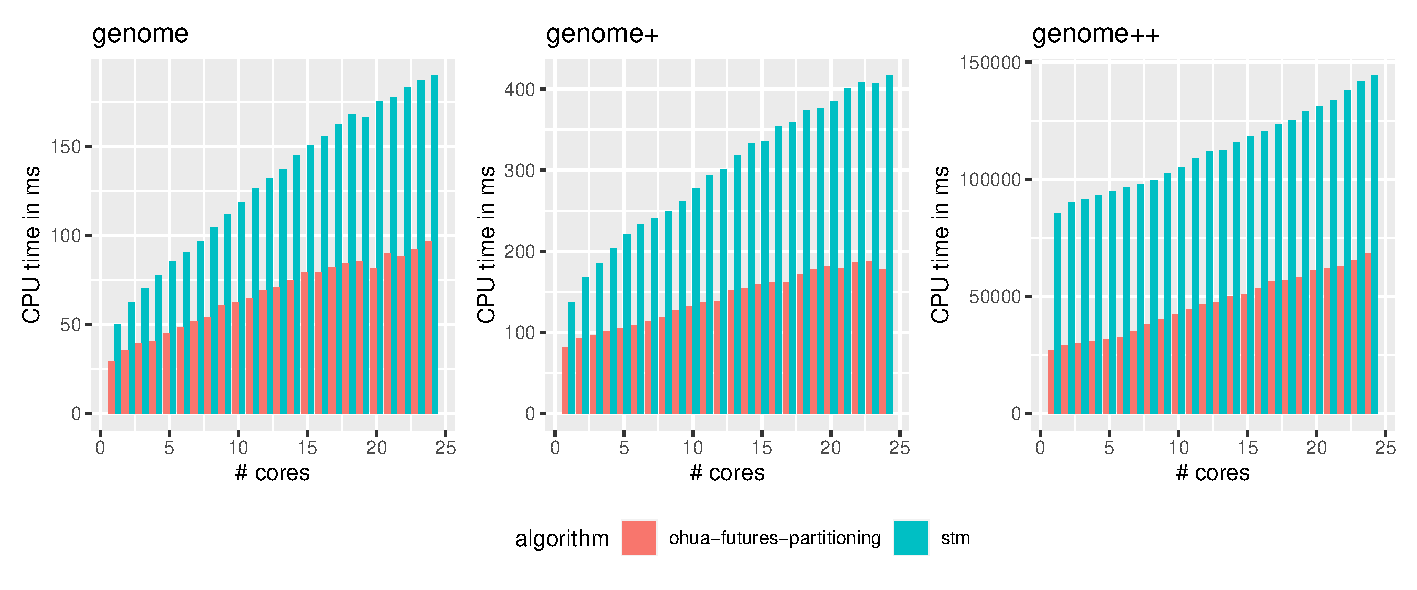
\includegraphics[width=\textwidth,keepaspectratio]{gfx/results/cpu_genome_comb}
    \caption{CPU time used by both frameworks in the genome application.}%
    \label{fig:evaluation:genome-cpu}
\end{figure}

%\begin{figure}
    %\centering
    %\begin{subfigure}[t]{.32\textwidth}
        %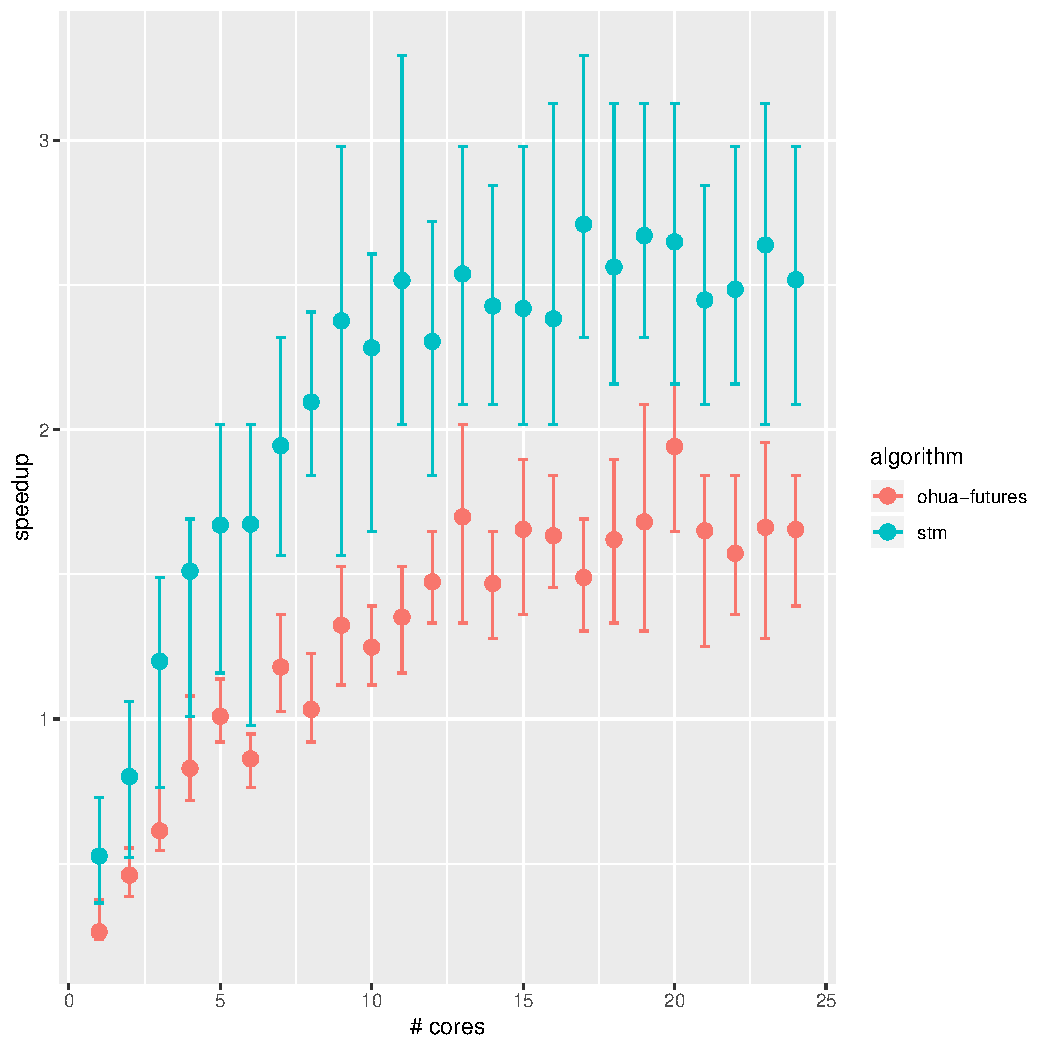
\includegraphics[width=\textwidth,keepaspectratio]{gfx/results/labyrinth/labyrinth}
        %\caption{labyrinth}%
    %\end{subfigure}%
    %~
    %\begin{subfigure}[t]{.32\textwidth}
        %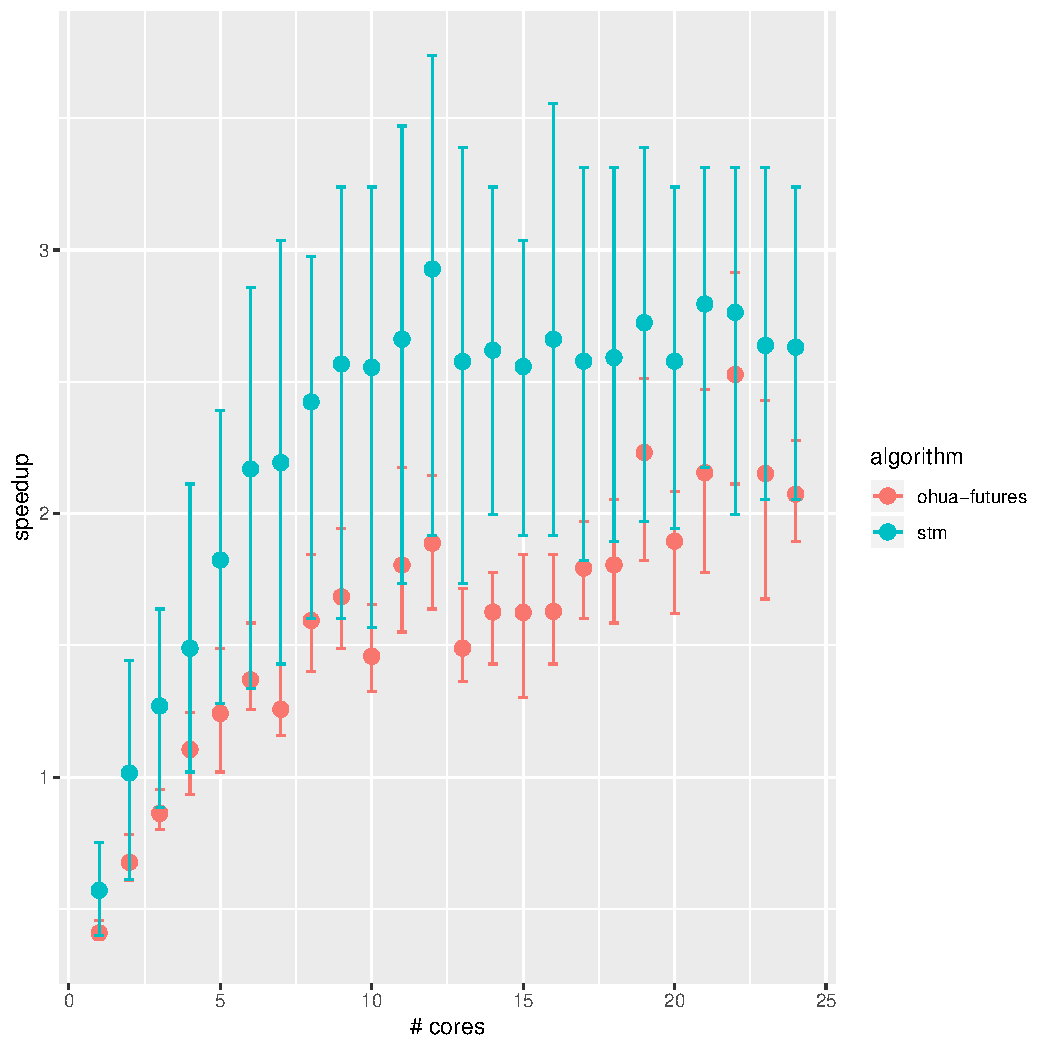
\includegraphics[width=\textwidth,keepaspectratio]{gfx/results/labyrinth/labyrinth+}
        %\caption{labyrinth+}%
    %\end{subfigure}%
    %~
    %\begin{subfigure}[t]{.32\textwidth}
        %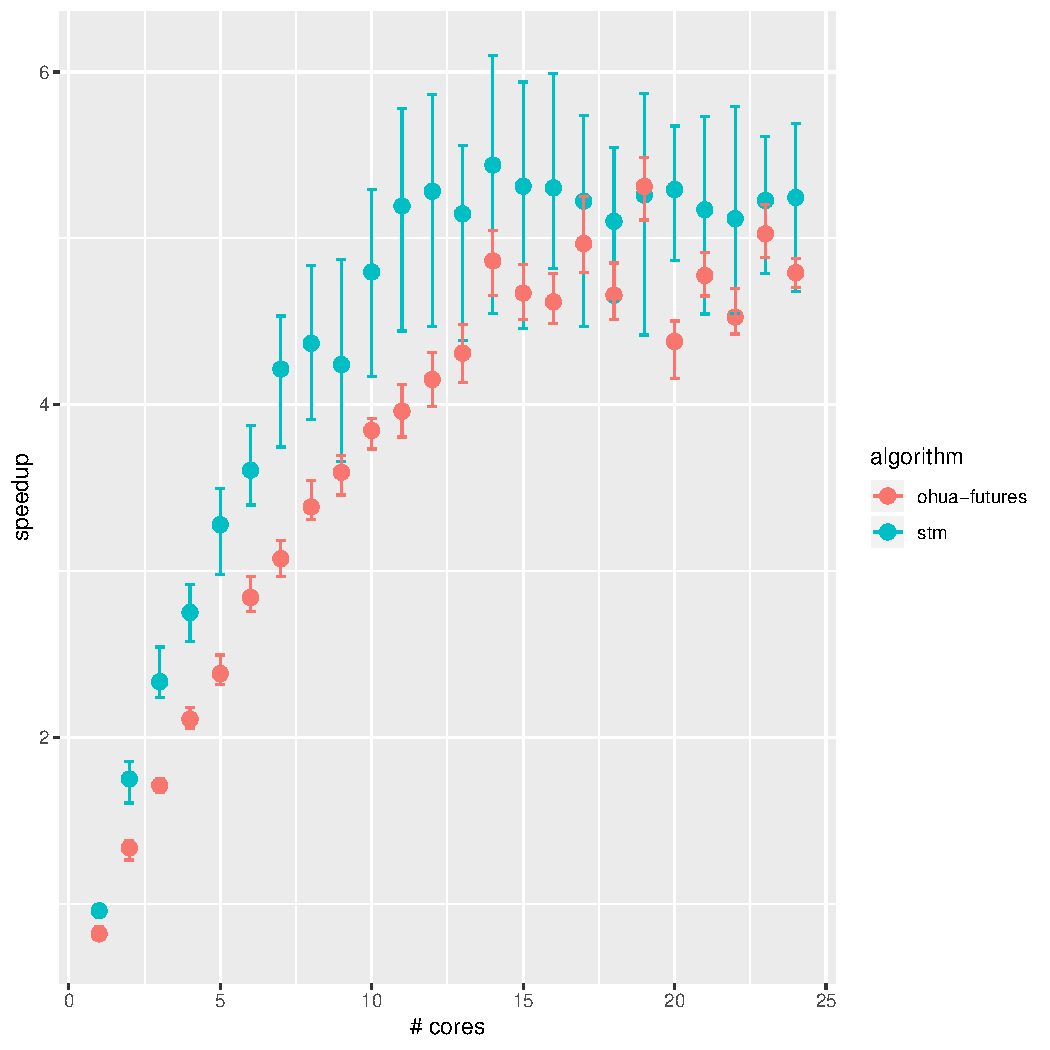
\includegraphics[width=\textwidth,keepaspectratio]{gfx/results/labyrinth/labyrinth++}
        %\caption{labyrinth++}%
    %\end{subfigure}%

    %\begin{subfigure}[t]{.32\textwidth}
        %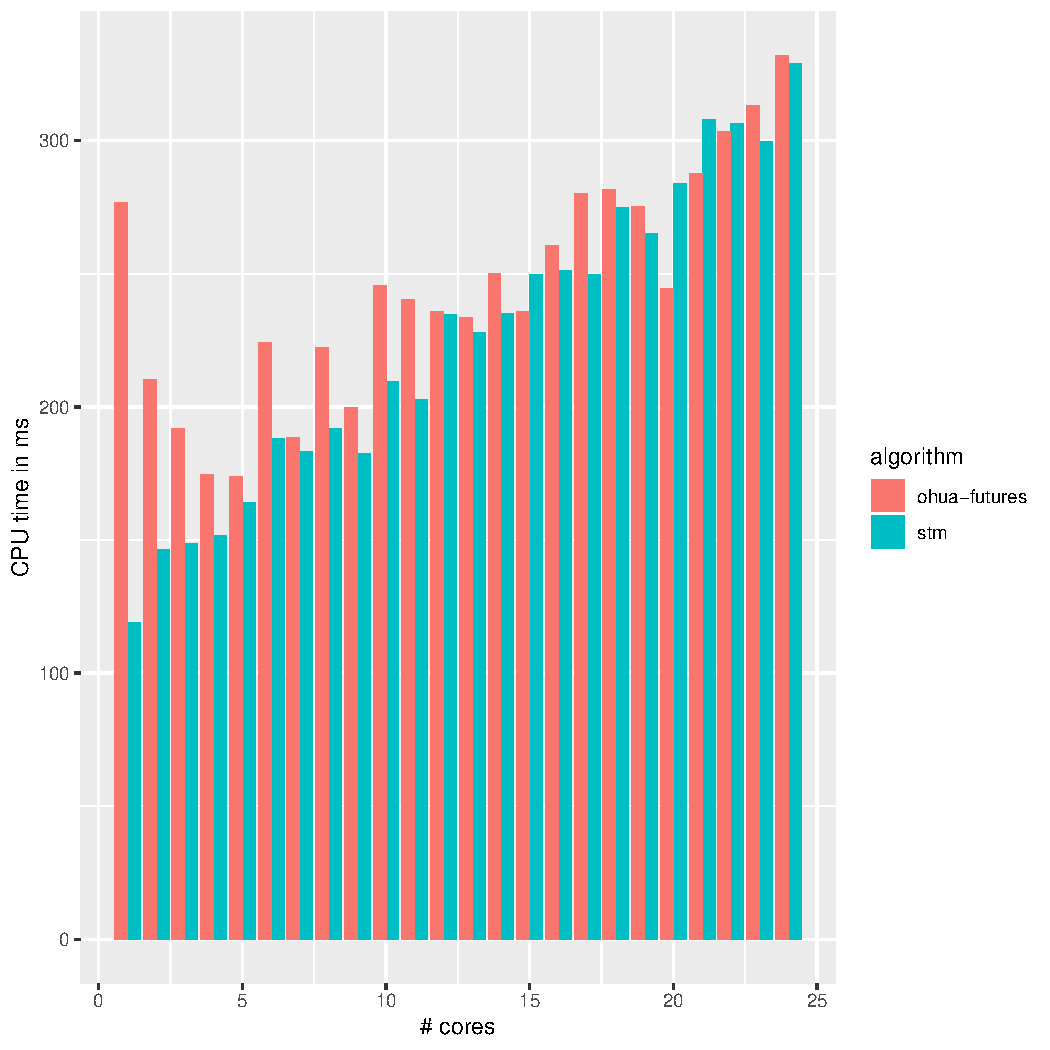
\includegraphics[width=\textwidth,keepaspectratio]{gfx/results/labyrinth/labyrinth_cpu}
        %\caption{cpu usage labyrinth}%
    %\end{subfigure}%
    %~
    %\begin{subfigure}[t]{.32\textwidth}
        %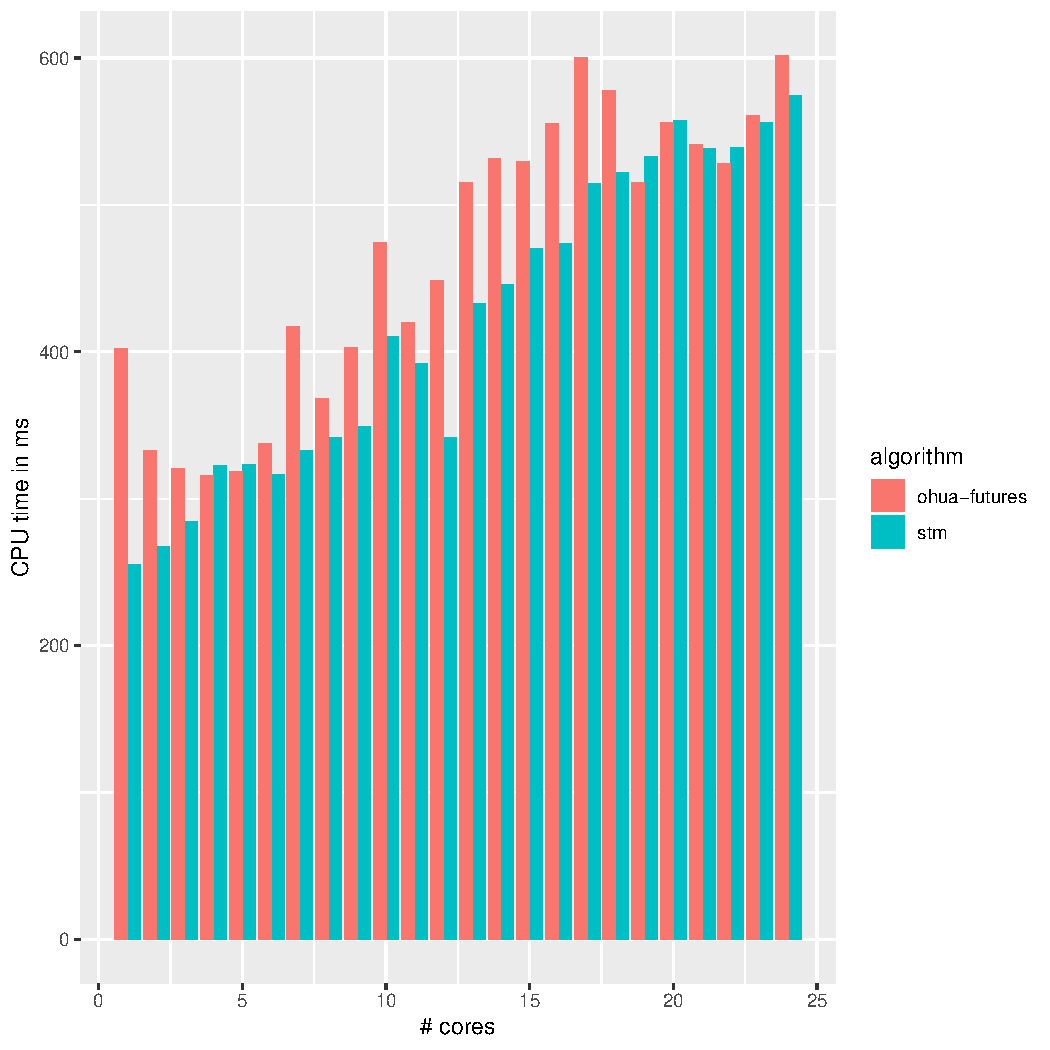
\includegraphics[width=\textwidth,keepaspectratio]{gfx/results/labyrinth/labyrinth+_cpu}
        %\caption{cpu usage labyrinth+}%
    %\end{subfigure}%
    %~
    %\begin{subfigure}[t]{.32\textwidth}
        %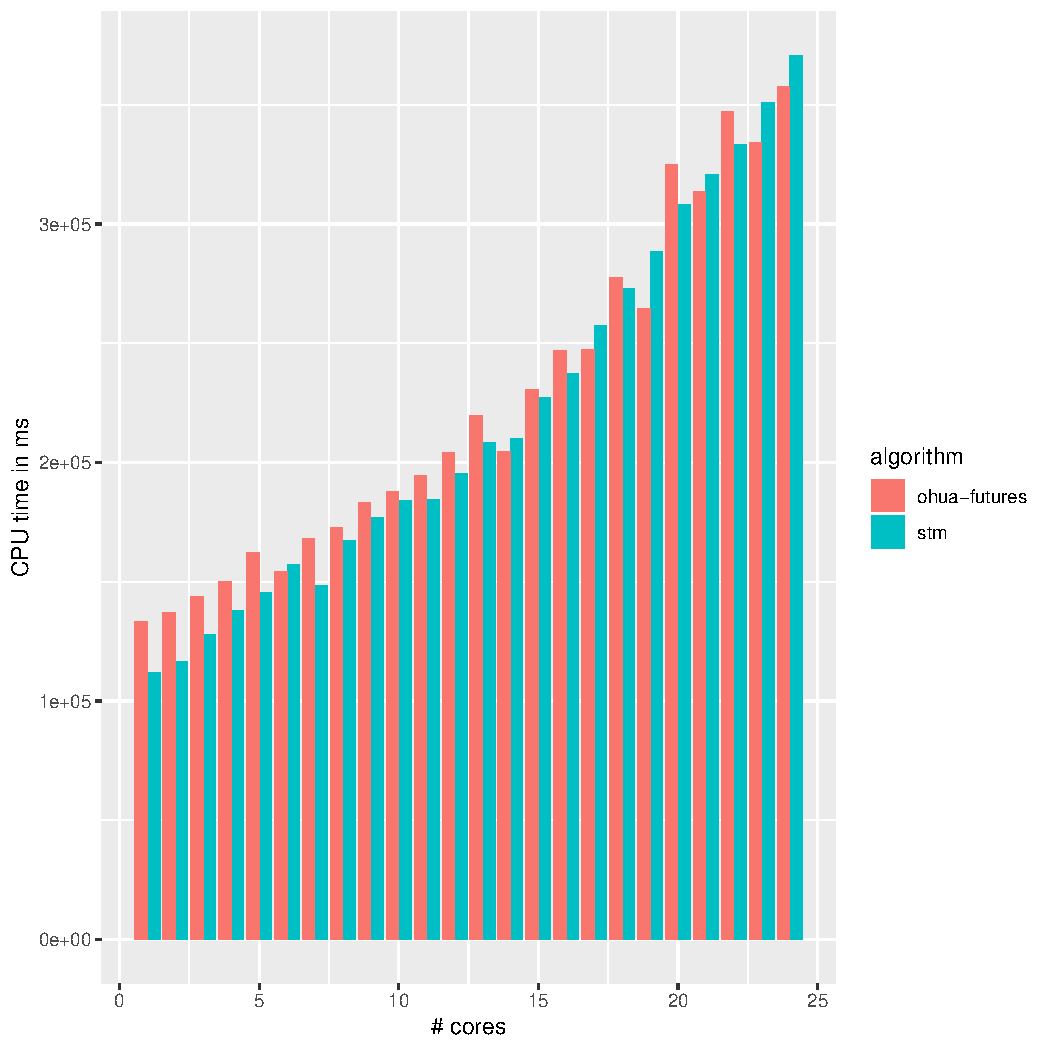
\includegraphics[width=\textwidth,keepaspectratio]{gfx/results/labyrinth/labyrinth++_cpu}
        %\caption{cpu usage labyrinth++}%
    %\end{subfigure}%
    %\caption{Results of the labyrinth benchmark.}%
    %\label{fig:evaulation:labyrinth}
%\end{figure}

%\begin{figure}
    %\centering
    %\begin{subfigure}[t]{.32\textwidth}
        %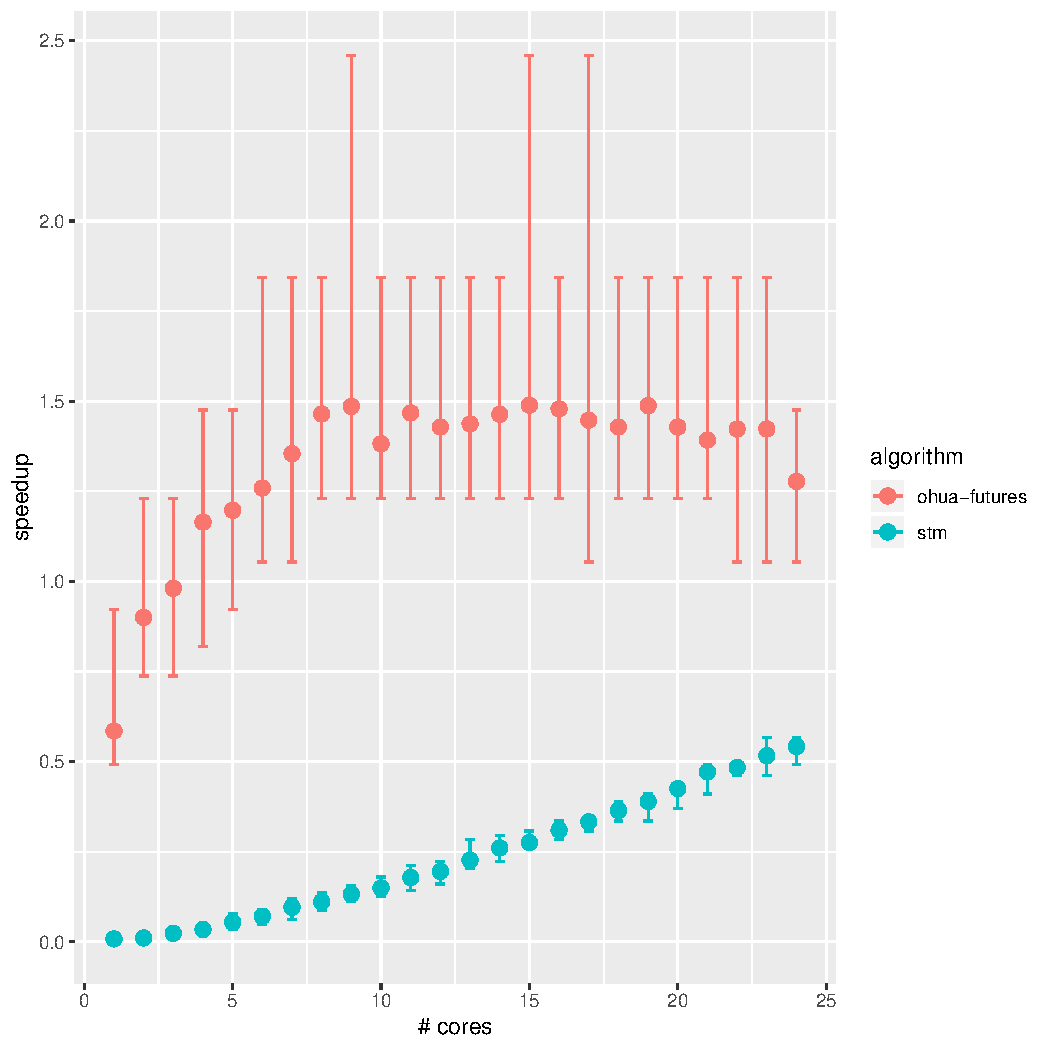
\includegraphics[width=\textwidth,keepaspectratio]{gfx/results/intruder/intruder}
        %\caption{intruder}%
    %\end{subfigure}%
    %~
    %\begin{subfigure}[t]{.32\textwidth}
        %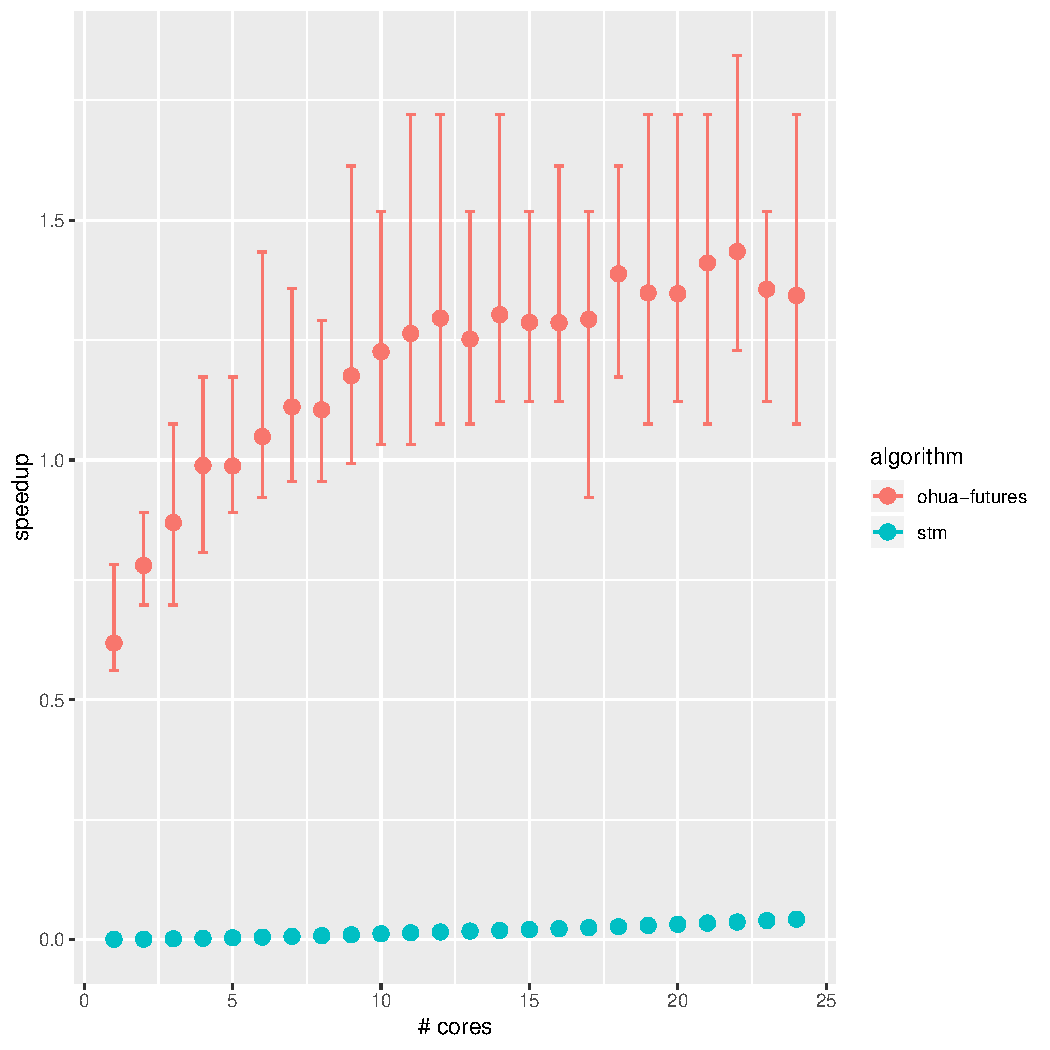
\includegraphics[width=\textwidth,keepaspectratio]{gfx/results/intruder/intruder+}
        %\caption{intruder+}%
    %\end{subfigure}%
    %% ~
    %% \begin{subfigure}[t]{.32\textwidth}
    %%     \includegraphics[width=\textwidth,keepaspectratio]{gfx/results/intruder/intruder++}
    %%     \caption{intruder++}%
    %% \end{subfigure}%

    %\begin{subfigure}[t]{.32\textwidth}
        %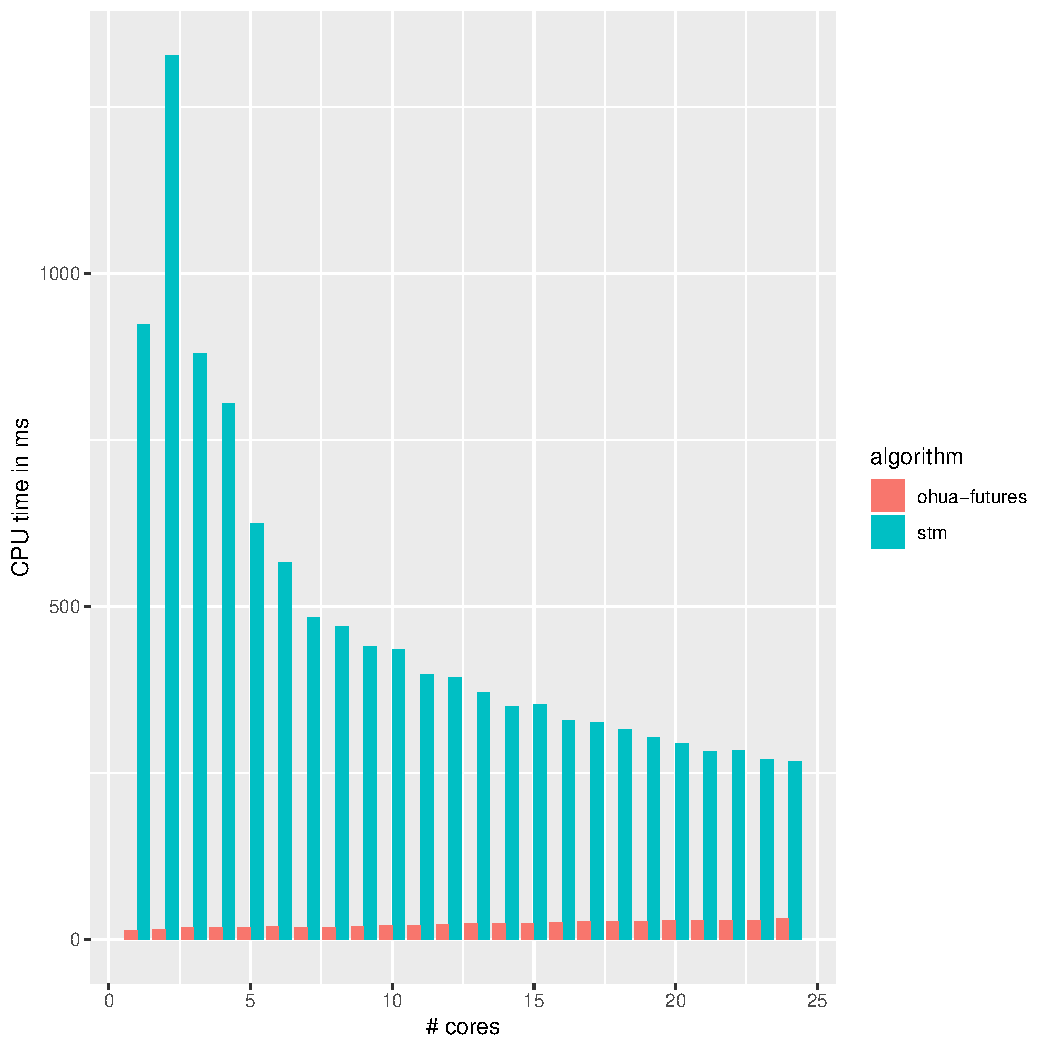
\includegraphics[width=\textwidth,keepaspectratio]{gfx/results/intruder/intruder_cpu}
        %\caption{cpu usage intruder}%
    %\end{subfigure}%
    %~
    %\begin{subfigure}[t]{.32\textwidth}
        %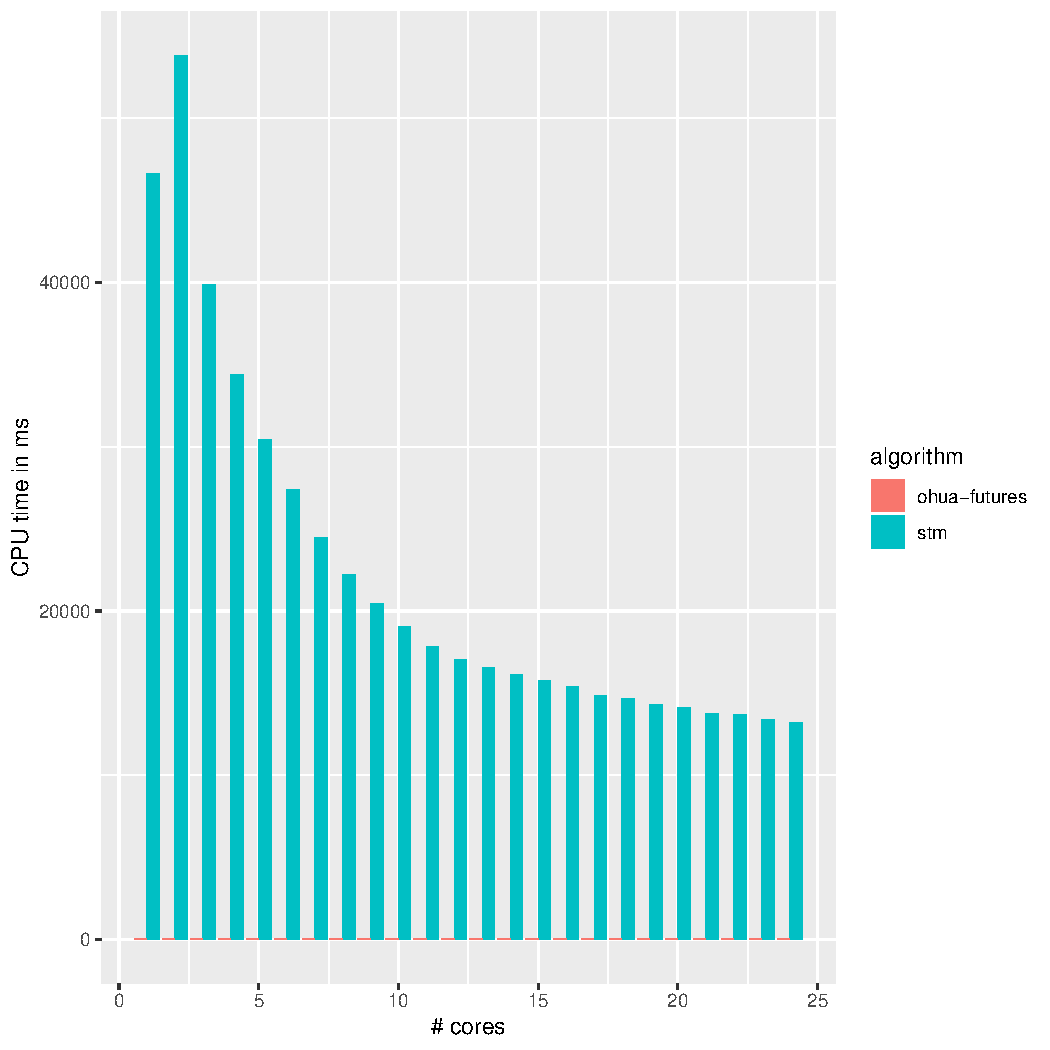
\includegraphics[width=\textwidth,keepaspectratio]{gfx/results/intruder/intruder+_cpu}
        %\caption{cpu usage intruder+}%
    %\end{subfigure}%
    %% ~
    %% \begin{subfigure}[t]{.32\textwidth}
    %%     \includegraphics[width=\textwidth,keepaspectratio]{gfx/results/intruder/intruder++_cpu}
    %%     \caption{cpu usage intruder++}%
    %% \end{subfigure}%
    %\caption{Results of the intruder benchmark.}%
    %\label{fig:evaulation:intruder}
%\end{figure}

%\begin{figure}
    %\centering
    %\begin{subfigure}[t]{.32\textwidth}
        %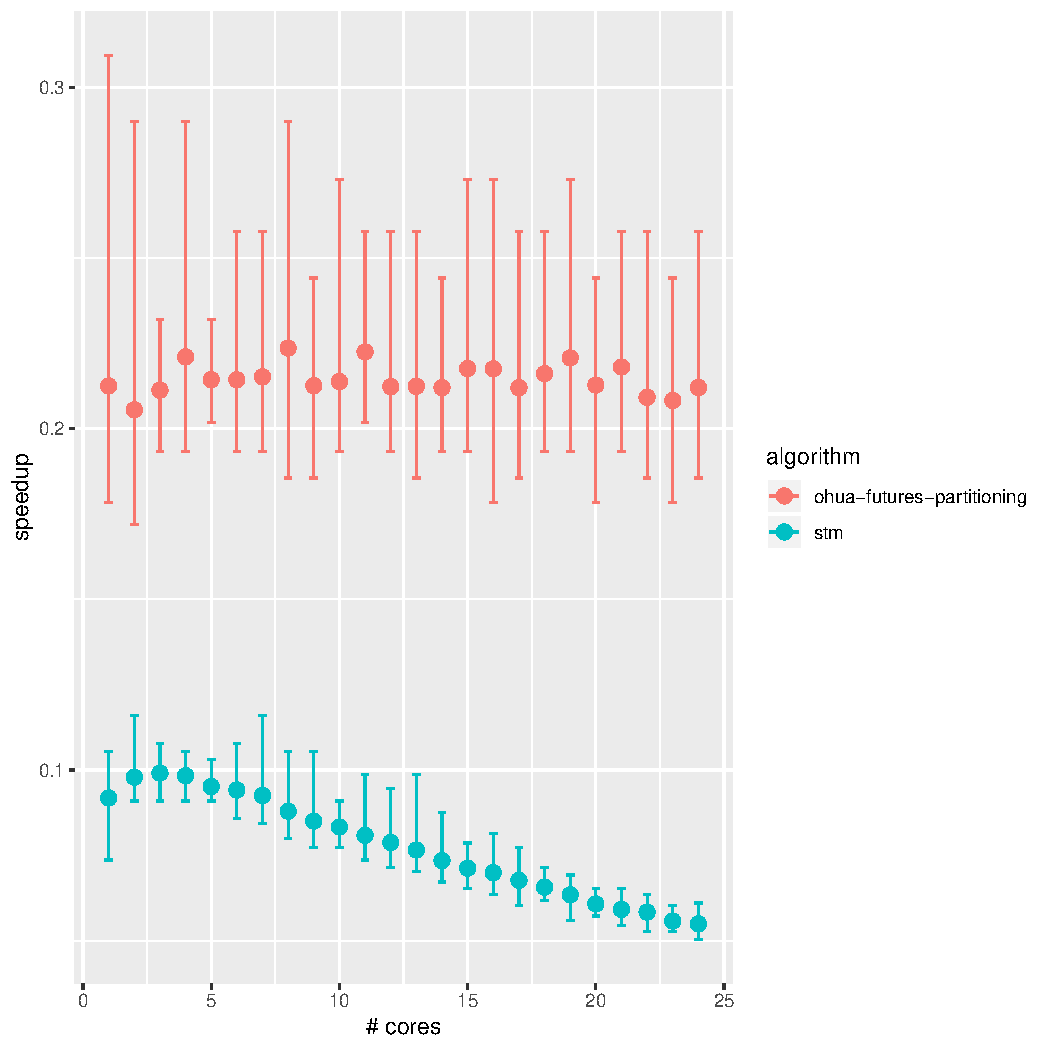
\includegraphics[width=\textwidth,keepaspectratio]{gfx/results/genome/genome}
        %\caption{genome}%
    %\end{subfigure}%
    %~
    %\begin{subfigure}[t]{.32\textwidth}
        %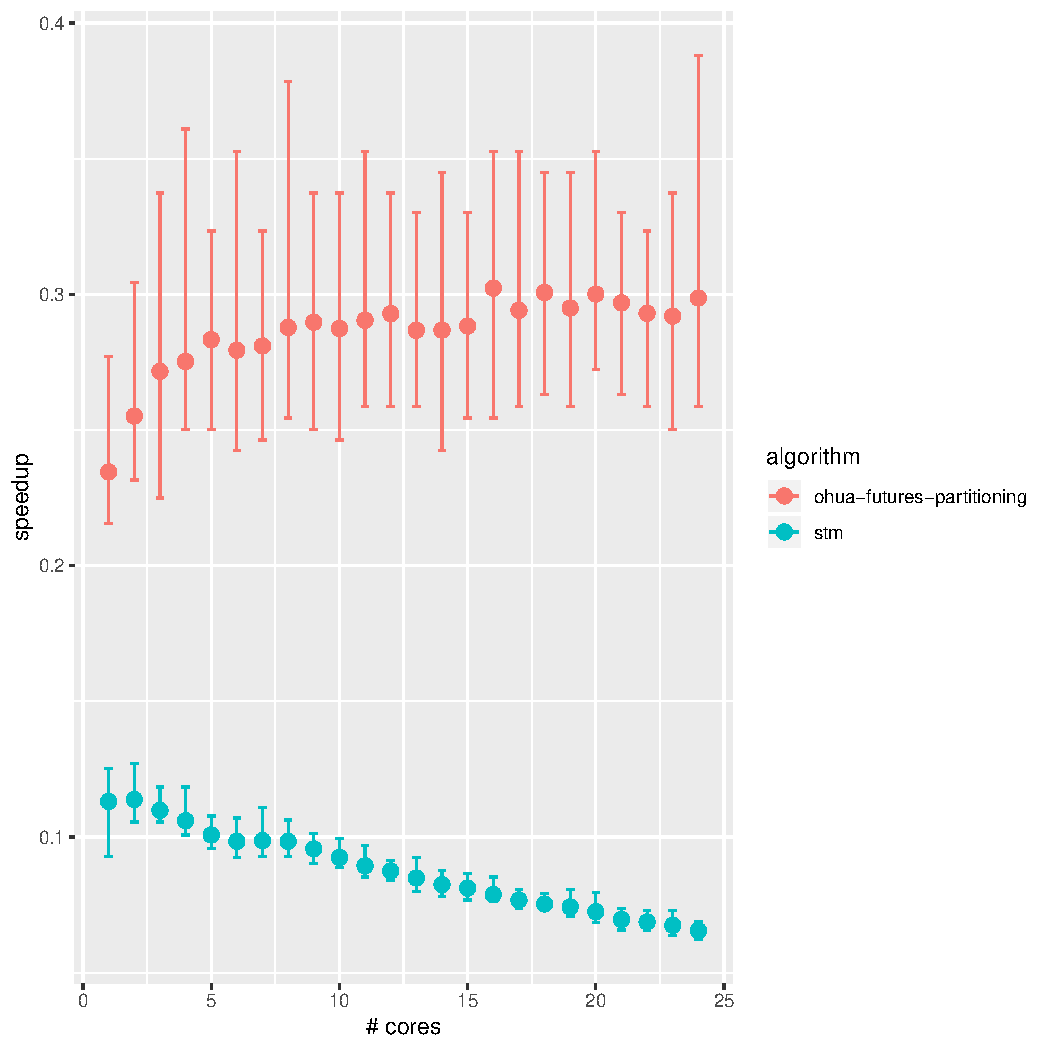
\includegraphics[width=\textwidth,keepaspectratio]{gfx/results/genome/genome+}
        %\caption{genome+}%
    %\end{subfigure}%
    %~
    %\begin{subfigure}[t]{.32\textwidth}
        %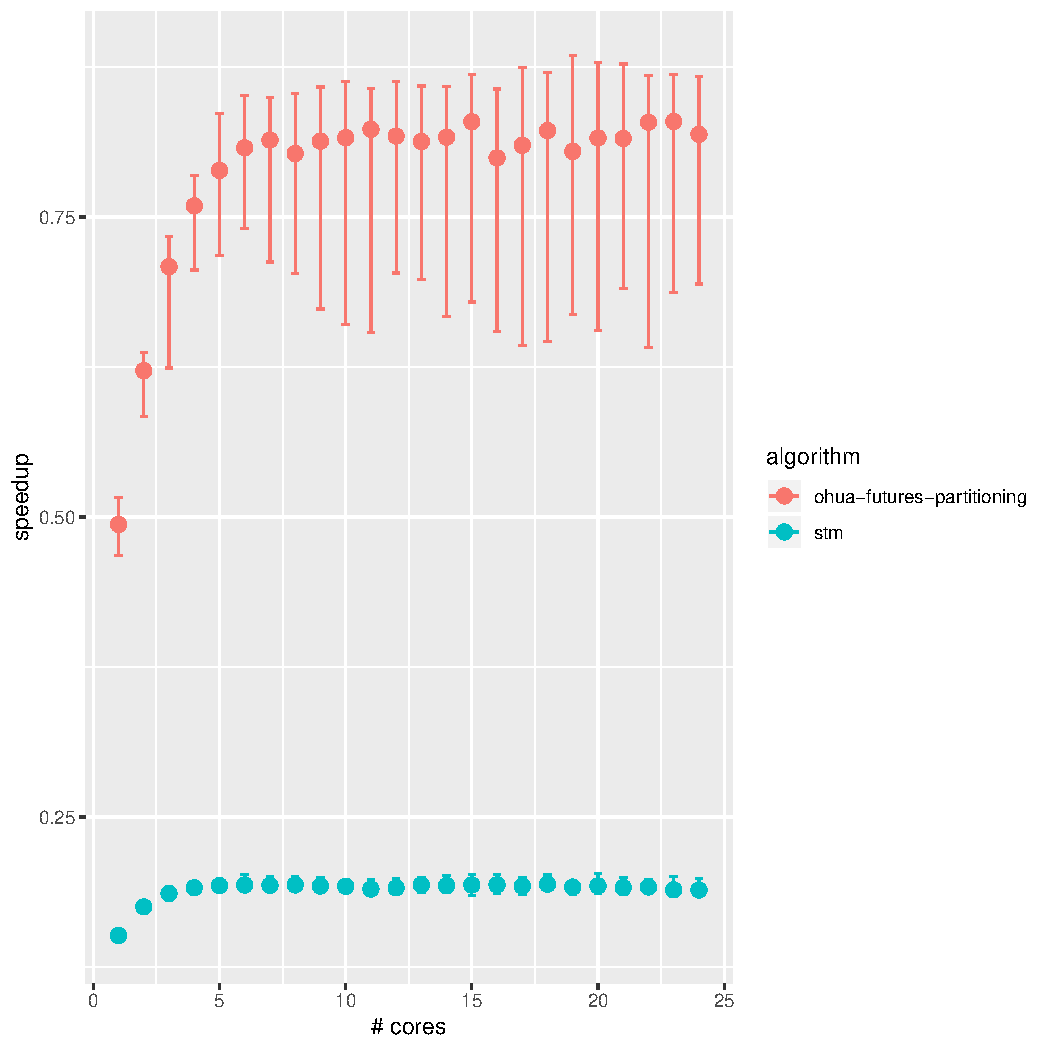
\includegraphics[width=\textwidth,keepaspectratio]{gfx/results/genome/genome++}
        %\caption{genome++}%
    %\end{subfigure}%

    %\begin{subfigure}[t]{.32\textwidth}
        %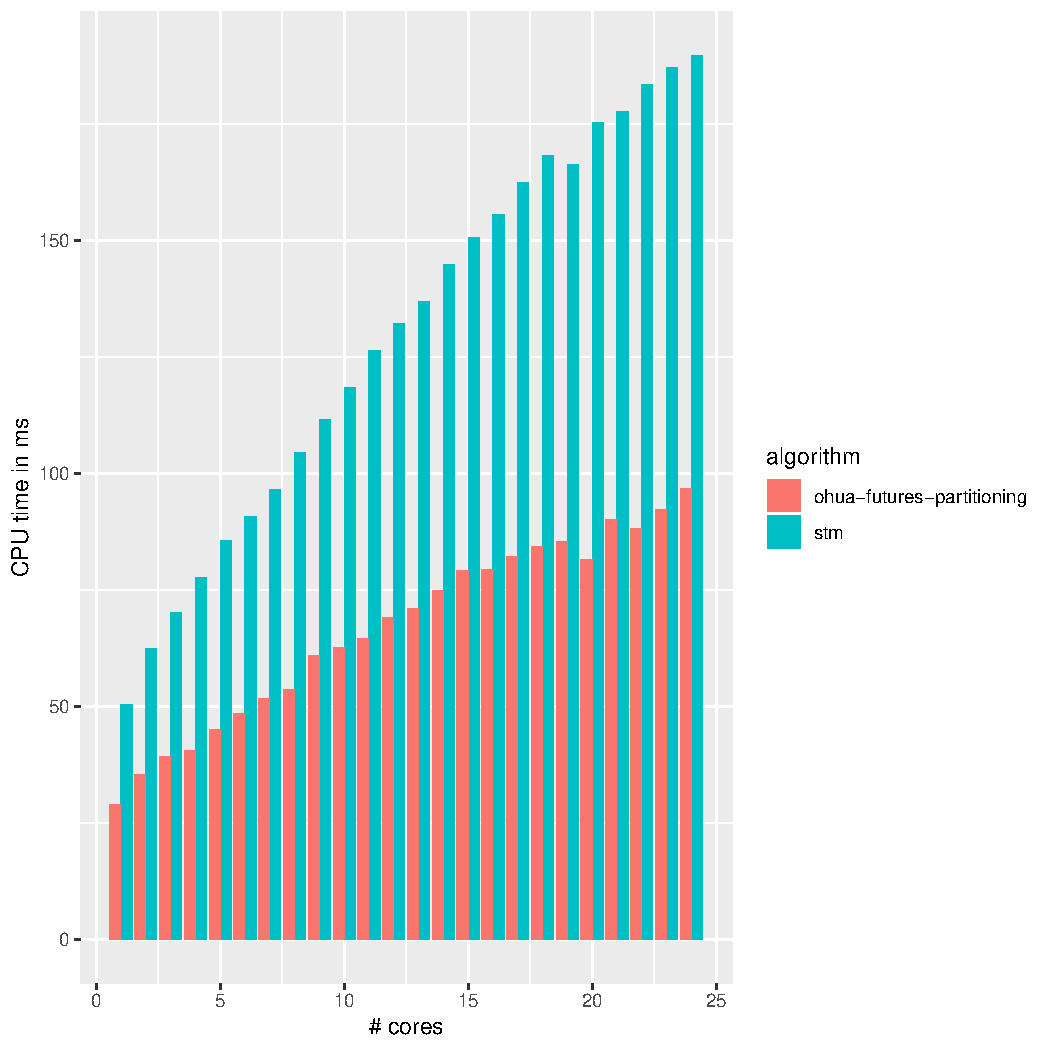
\includegraphics[width=\textwidth,keepaspectratio]{gfx/results/genome/genome_cpu}
        %\caption{cpu usage genome}%
    %\end{subfigure}%
    %~
    %\begin{subfigure}[t]{.32\textwidth}
        %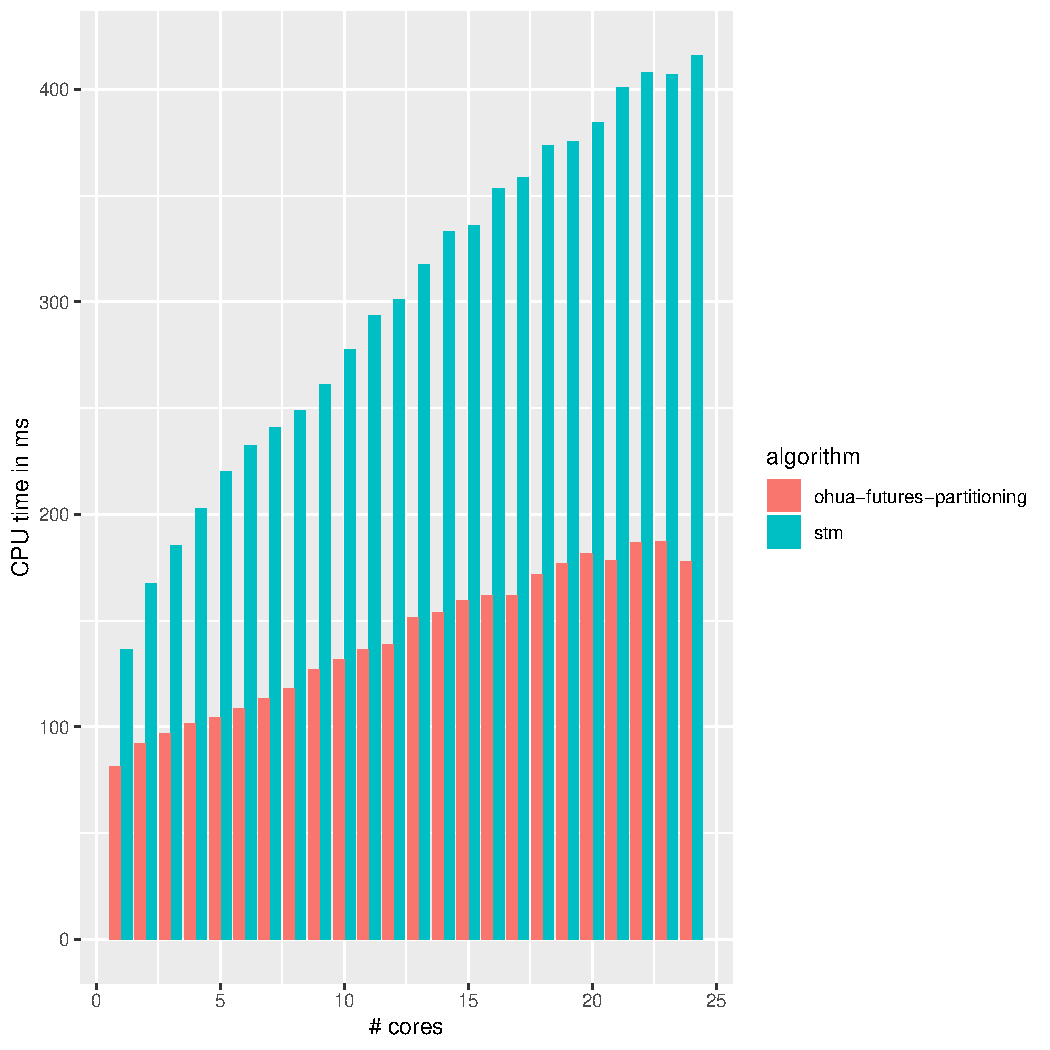
\includegraphics[width=\textwidth,keepaspectratio]{gfx/results/genome/genome+_cpu}
        %\caption{cpu usage genome+}%
    %\end{subfigure}%
    %~
    %\begin{subfigure}[t]{.32\textwidth}
        %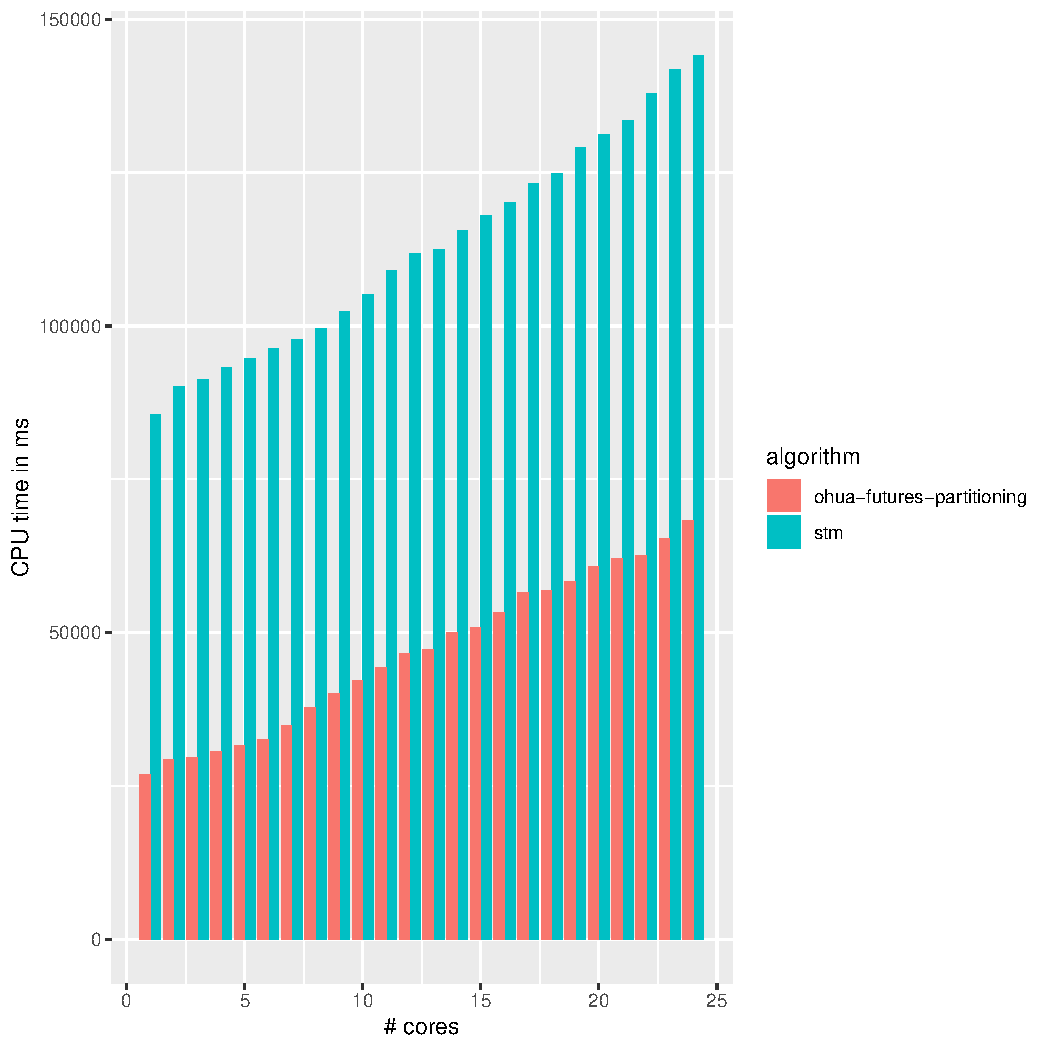
\includegraphics[width=\textwidth,keepaspectratio]{gfx/results/genome/genome++_cpu}
        %\caption{cpu usage genome++}%
    %\end{subfigure}%
    %\caption{Results of the genome benchmark.}%
    %\label{fig:evaulation:genome}
%\end{figure}

%\begin{figure}
    %\begin{subfigure}[t]{.32\textwidth}
        %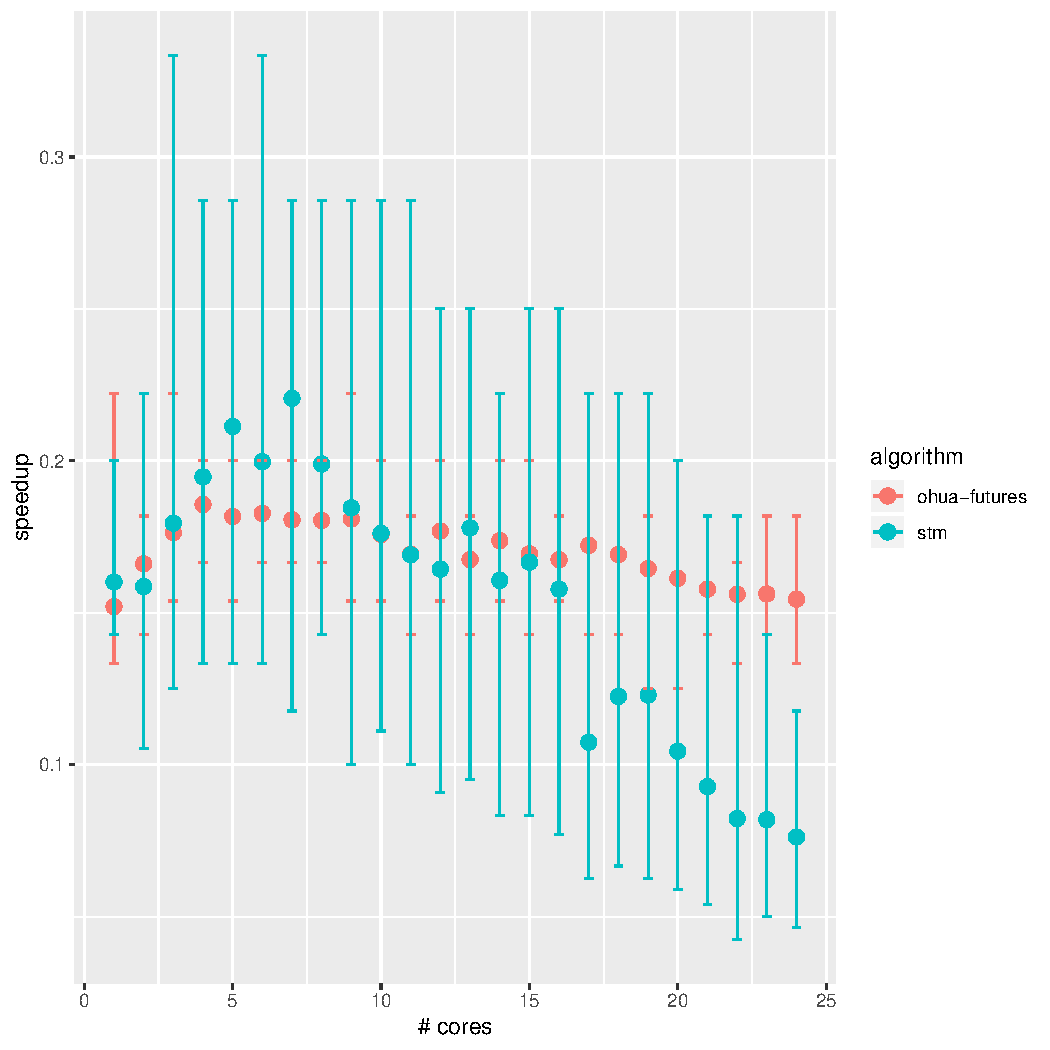
\includegraphics[width=\textwidth,keepaspectratio]{gfx/results/kmeans/kmeans-high}
        %\caption{kmeans-high}%
    %\end{subfigure}%
    %~
    %\begin{subfigure}[t]{.32\textwidth}
        %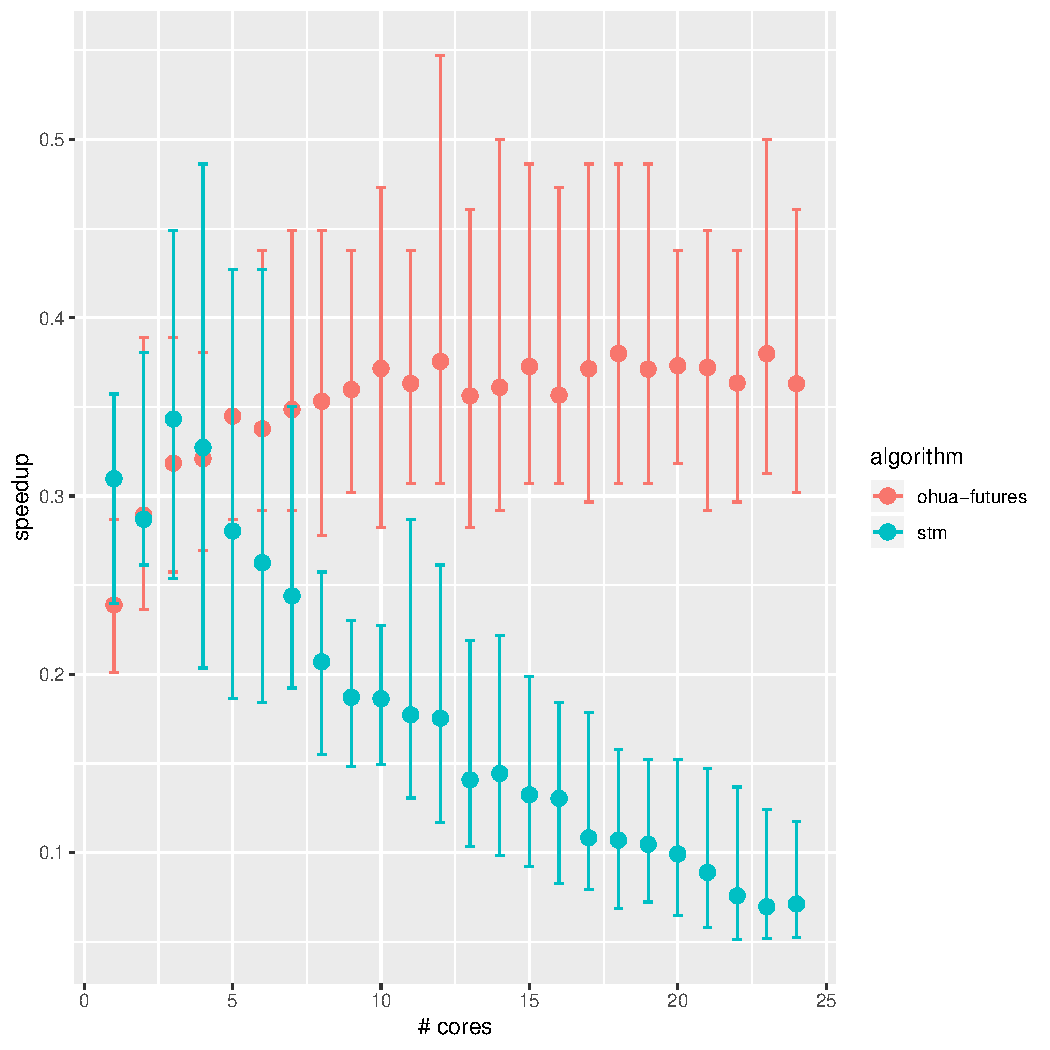
\includegraphics[width=\textwidth,keepaspectratio]{gfx/results/kmeans/kmeans-high+}
        %\caption{kmeans-high+}%
    %\end{subfigure}%
    %~
    %\begin{subfigure}[t]{.32\textwidth}
        %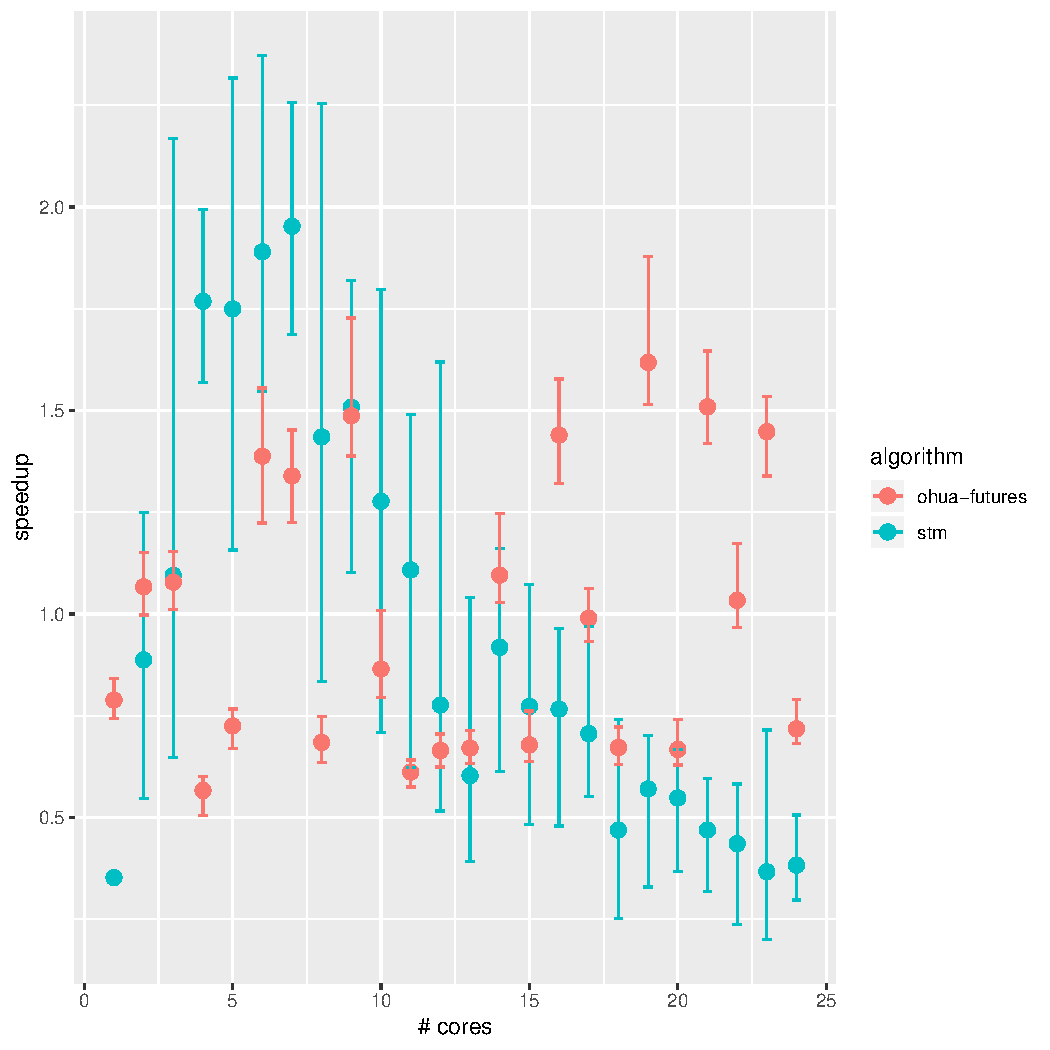
\includegraphics[width=\textwidth,keepaspectratio]{gfx/results/kmeans/kmeans-high++}
        %\caption{kmeans-high++}%
    %\end{subfigure}%

    %\begin{subfigure}[t]{.32\textwidth}
        %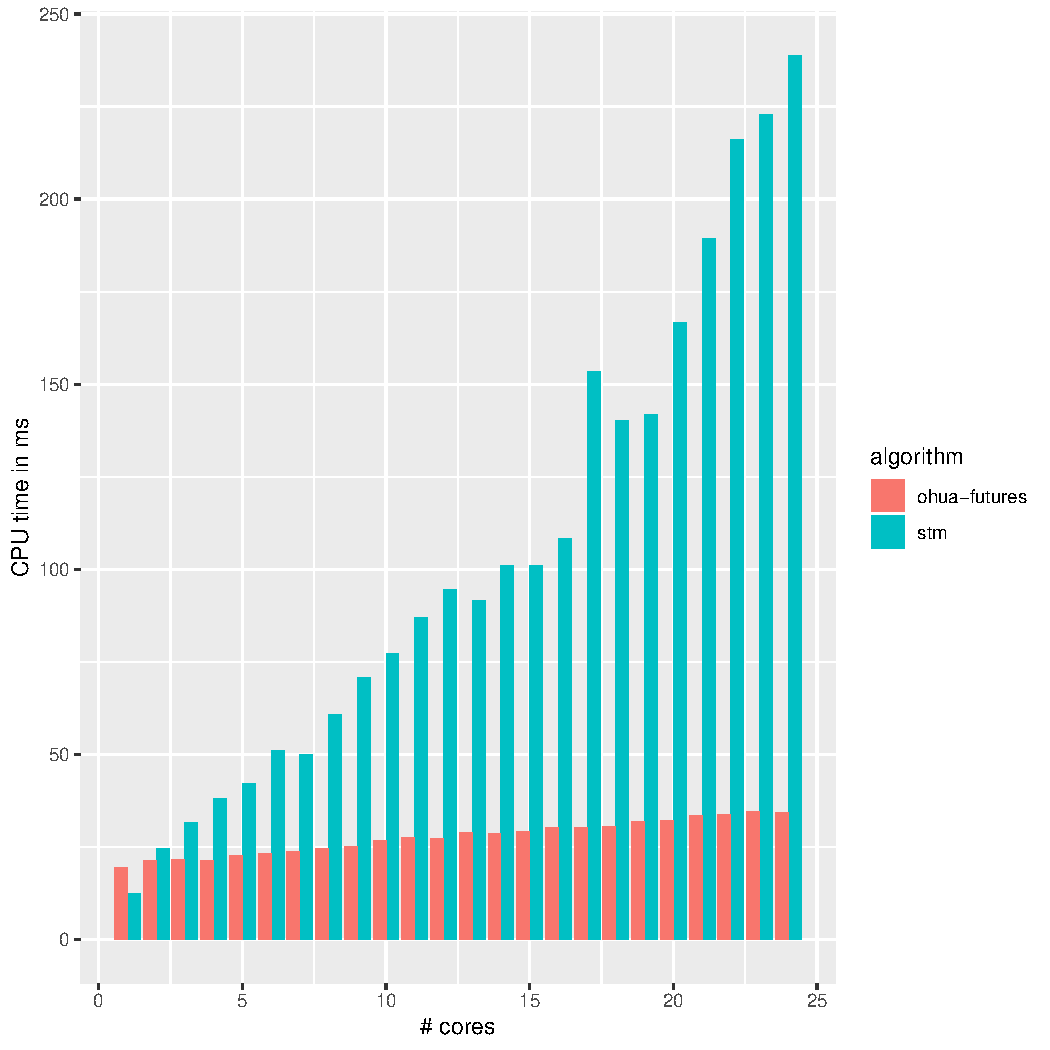
\includegraphics[width=\textwidth,keepaspectratio]{gfx/results/kmeans/kmeans-high_cpu}
        %\caption{cpu usage kmeans-high}%
    %\end{subfigure}%
    %~
    %\begin{subfigure}[t]{.32\textwidth}
        %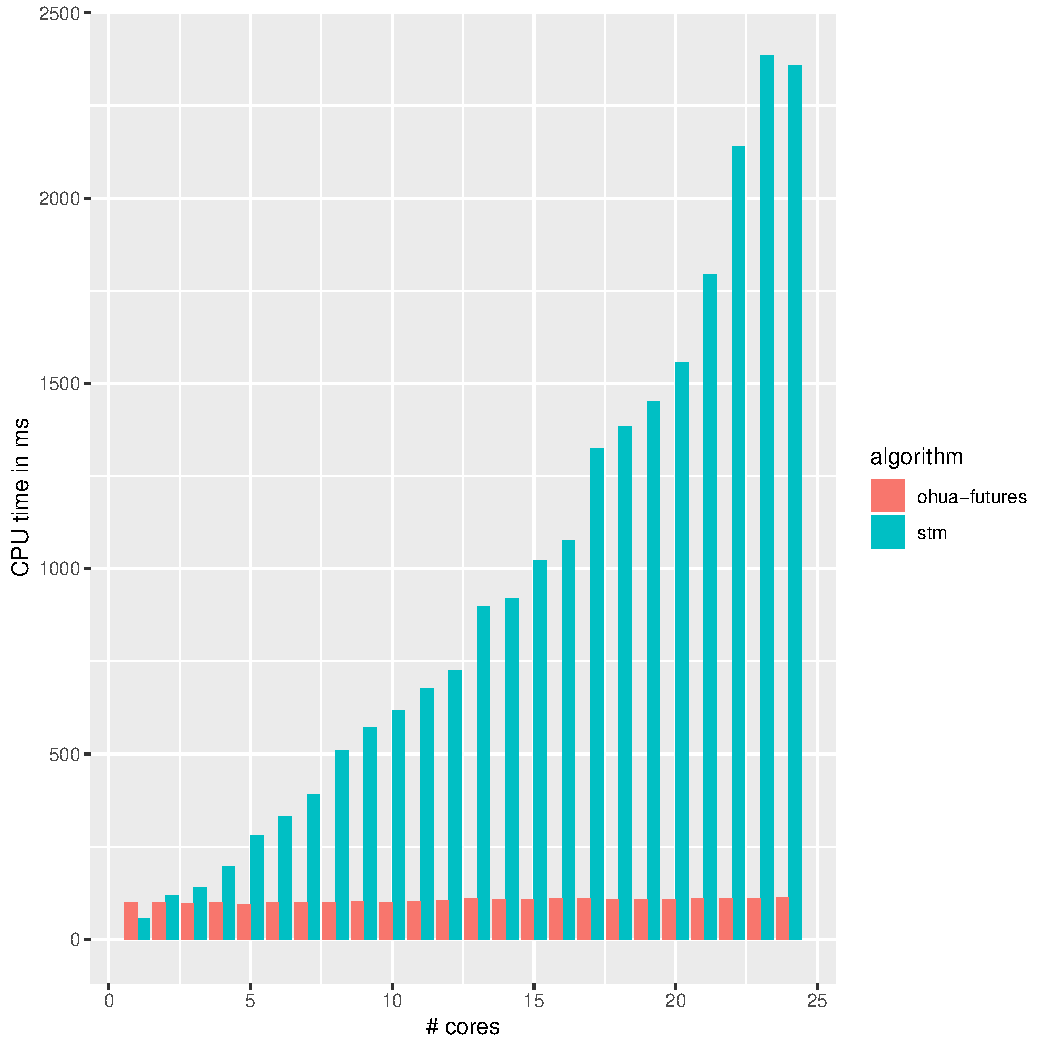
\includegraphics[width=\textwidth,keepaspectratio]{gfx/results/kmeans/kmeans-high+_cpu}
        %\caption{cpu usage kmeans-high+}%
    %\end{subfigure}%
    %~
    %\begin{subfigure}[t]{.32\textwidth}
        %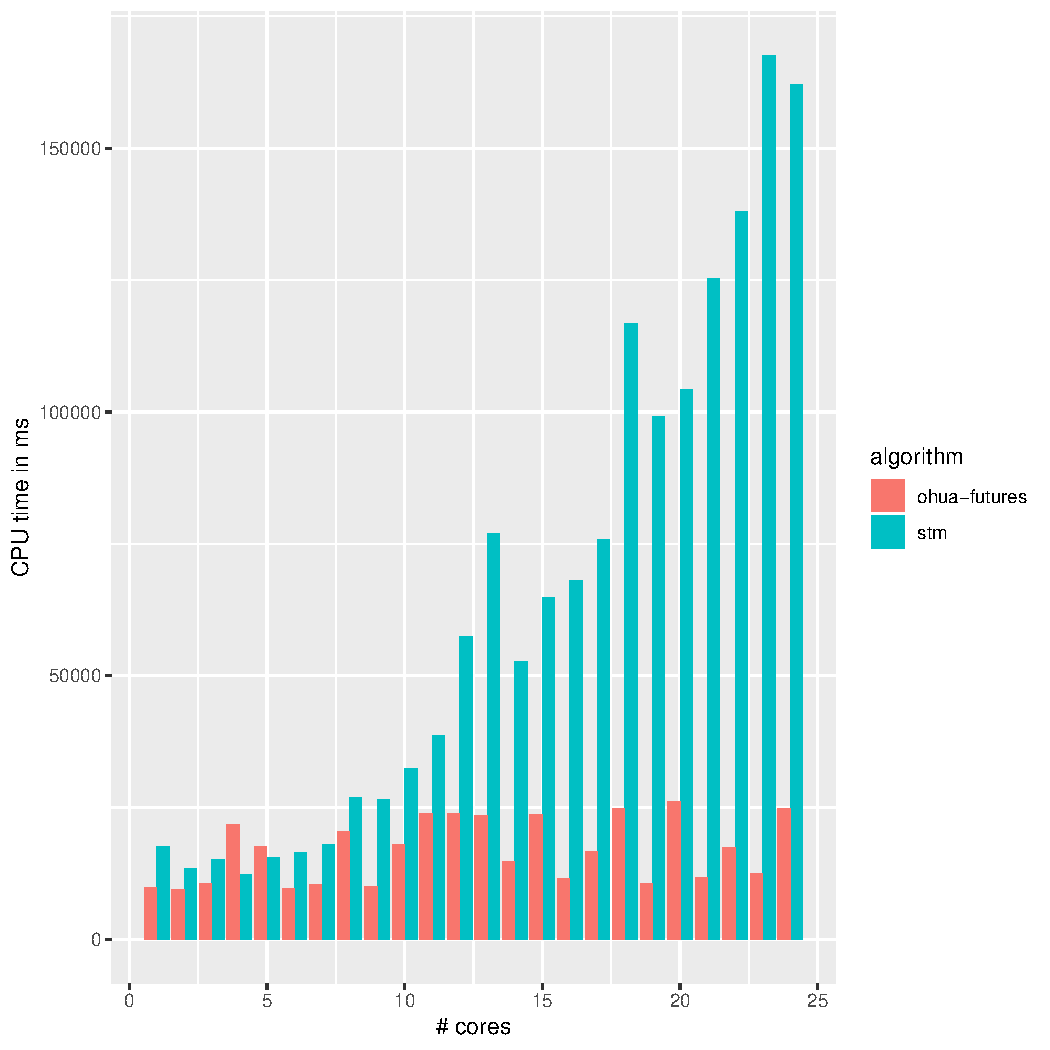
\includegraphics[width=\textwidth,keepaspectratio]{gfx/results/kmeans/kmeans-high++_cpu}
        %\caption{cpu usage kmeans-high++}%
    %\end{subfigure}%
    %\caption{Results of the kmeans-high benchmark.}%
    %\label{fig:evaulation:kmeans-high}
%\end{figure}

%\begin{figure}
    %\begin{subfigure}[t]{.32\textwidth}
        %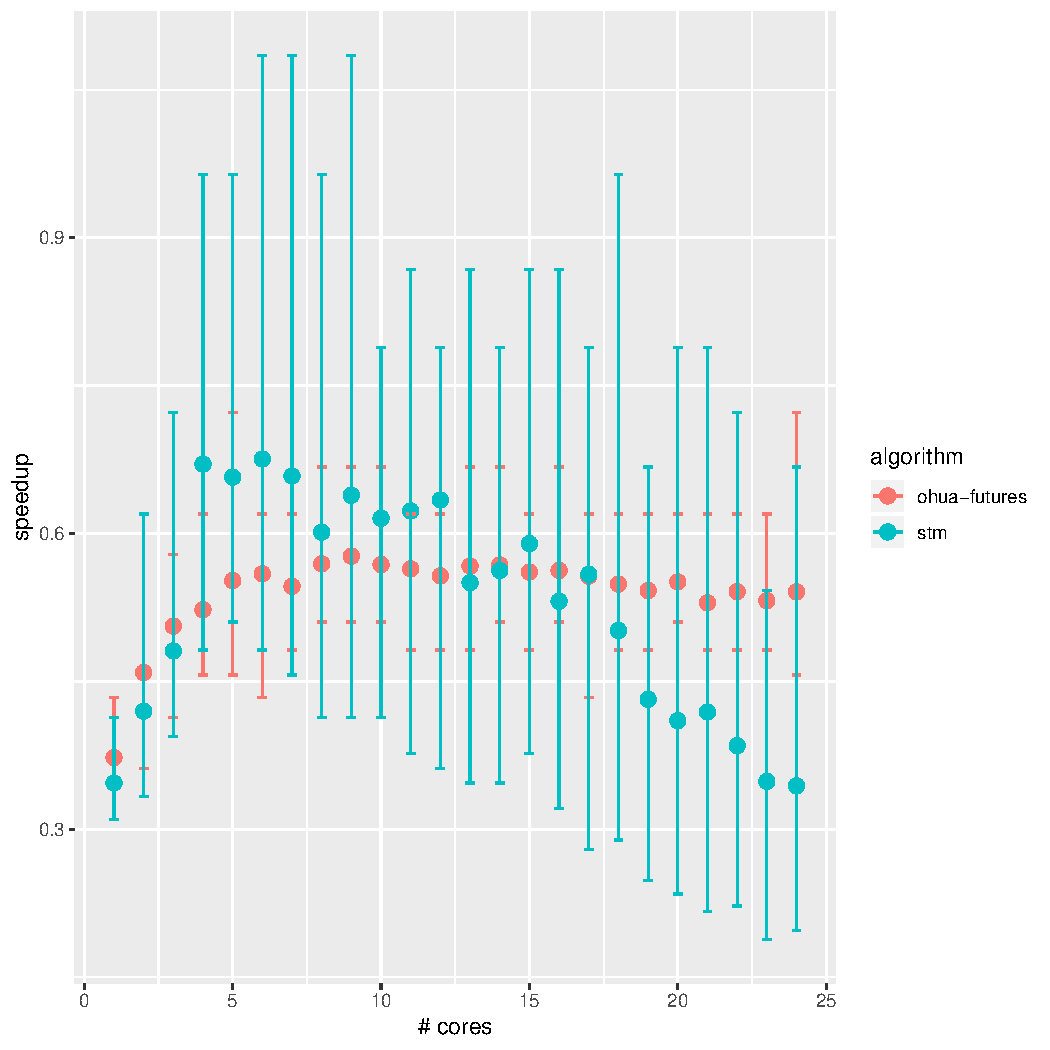
\includegraphics[width=\textwidth,keepaspectratio]{gfx/results/kmeans/kmeans-low}
        %\caption{kmeans-low}%
    %\end{subfigure}%
    %~
    %\begin{subfigure}[t]{.32\textwidth}
        %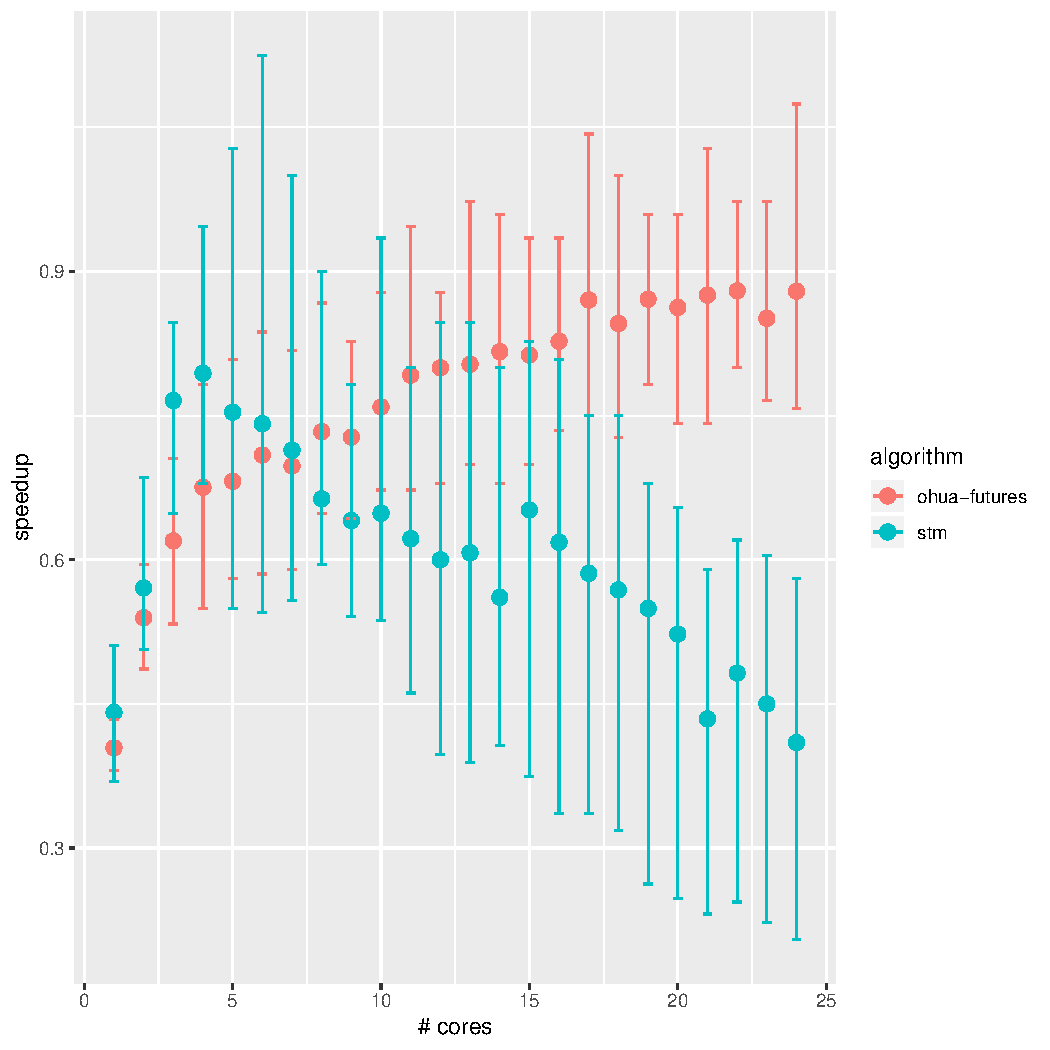
\includegraphics[width=\textwidth,keepaspectratio]{gfx/results/kmeans/kmeans-low+}
        %\caption{kmeans-low+}%
    %\end{subfigure}%
    %~
    %\begin{subfigure}[t]{.32\textwidth}
        %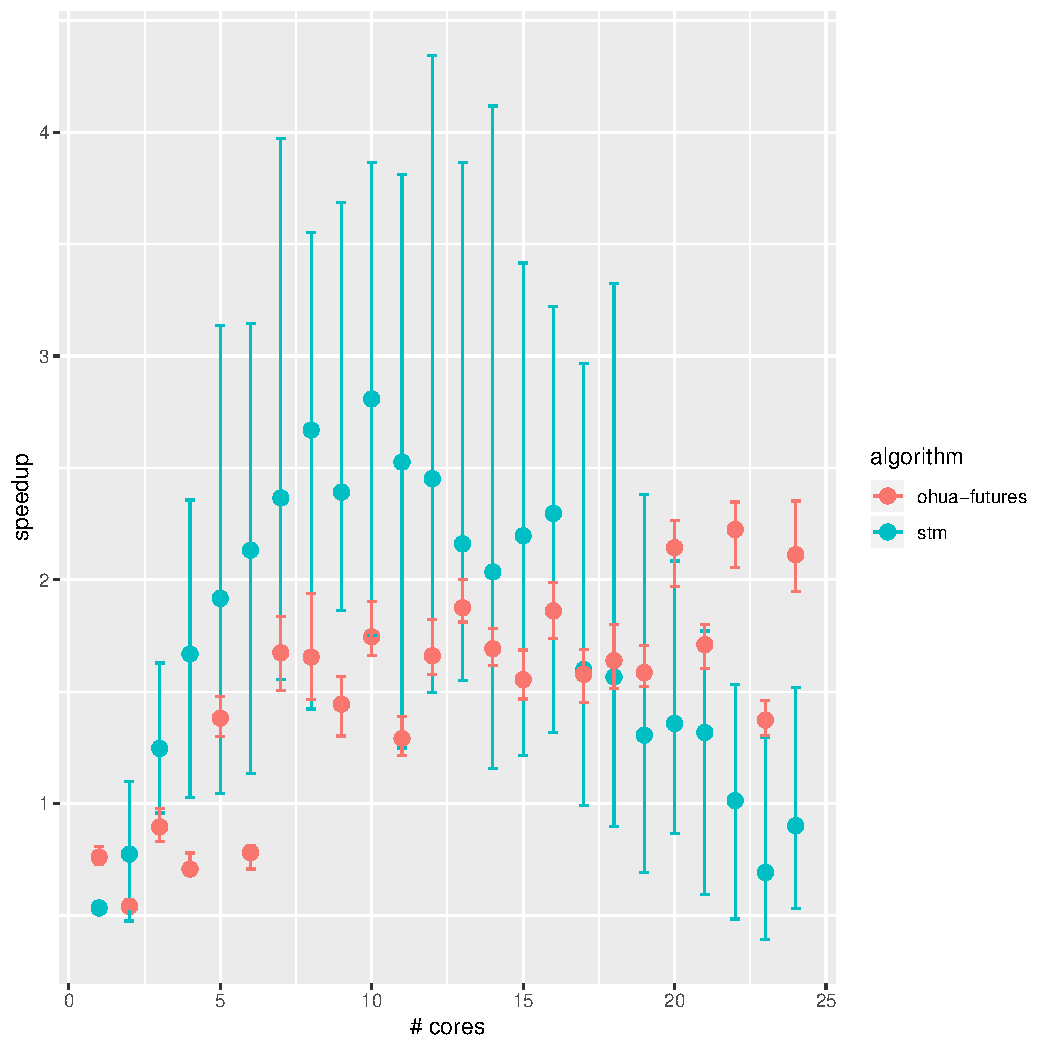
\includegraphics[width=\textwidth,keepaspectratio]{gfx/results/kmeans/kmeans-low++}
        %\caption{kmeans-low++}%
    %\end{subfigure}%

    %\begin{subfigure}[t]{.32\textwidth}
        %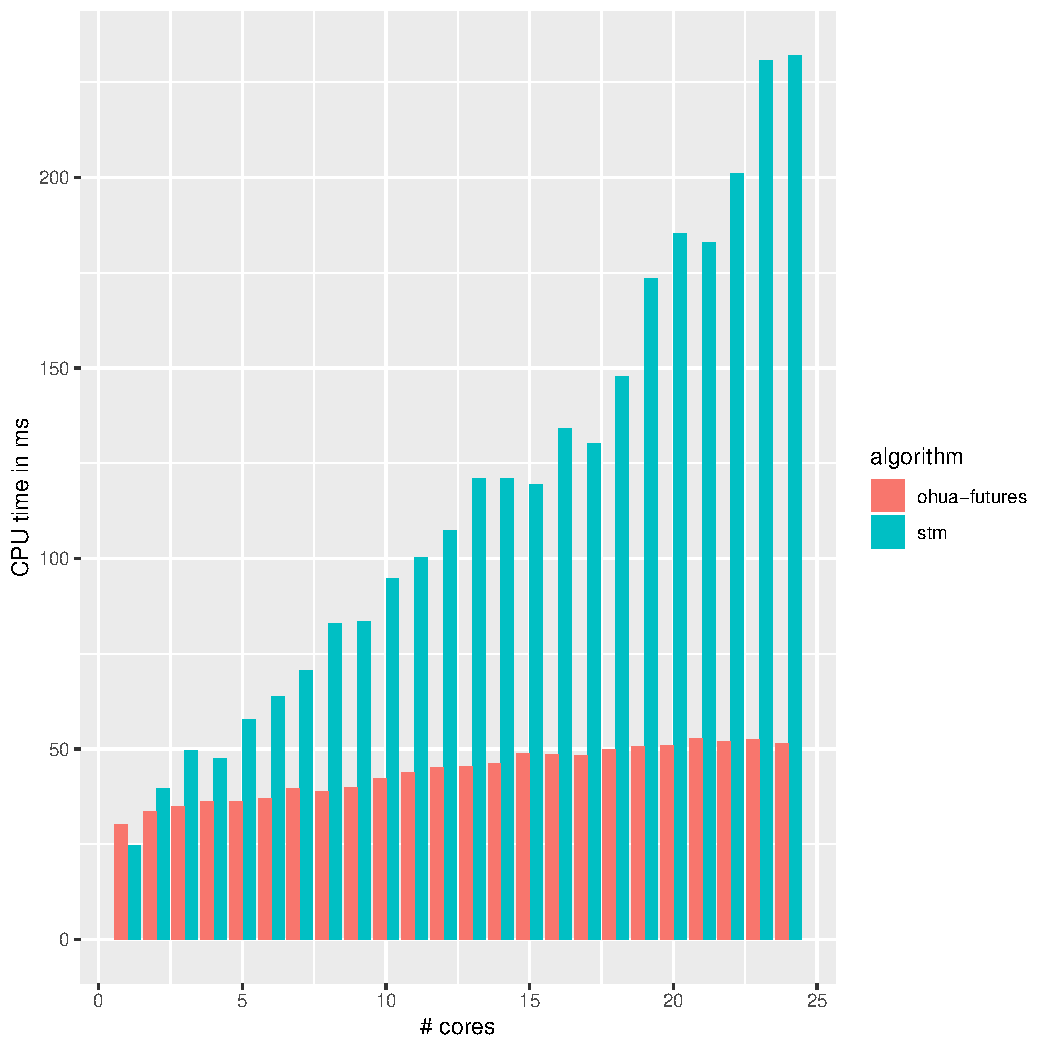
\includegraphics[width=\textwidth,keepaspectratio]{gfx/results/kmeans/kmeans-low_cpu}
        %\caption{cpu usage kmeans-low}%
    %\end{subfigure}%
    %~
    %\begin{subfigure}[t]{.32\textwidth}
        %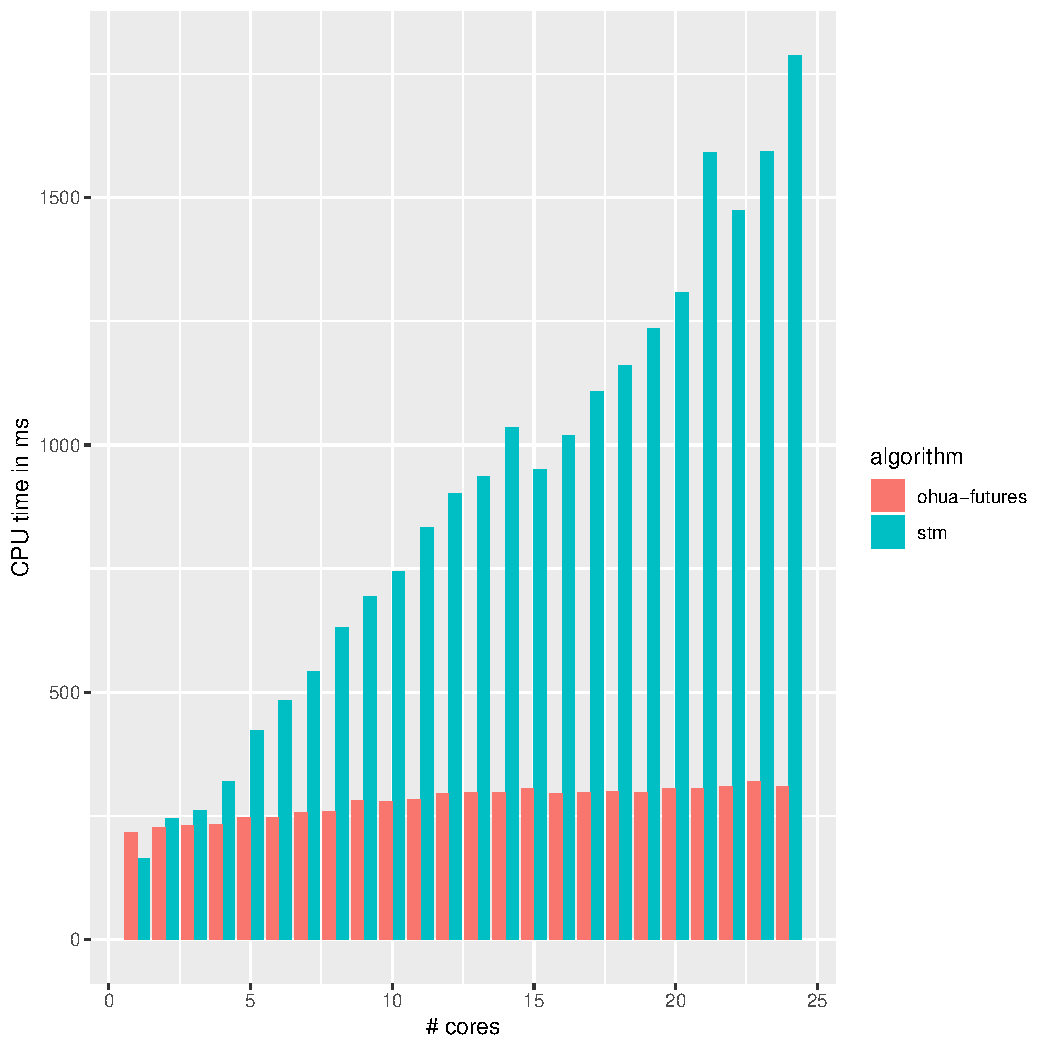
\includegraphics[width=\textwidth,keepaspectratio]{gfx/results/kmeans/kmeans-low+_cpu}
        %\caption{cpu usage kmeans-low+}%
    %\end{subfigure}%
    %~
    %\begin{subfigure}[t]{.32\textwidth}
        %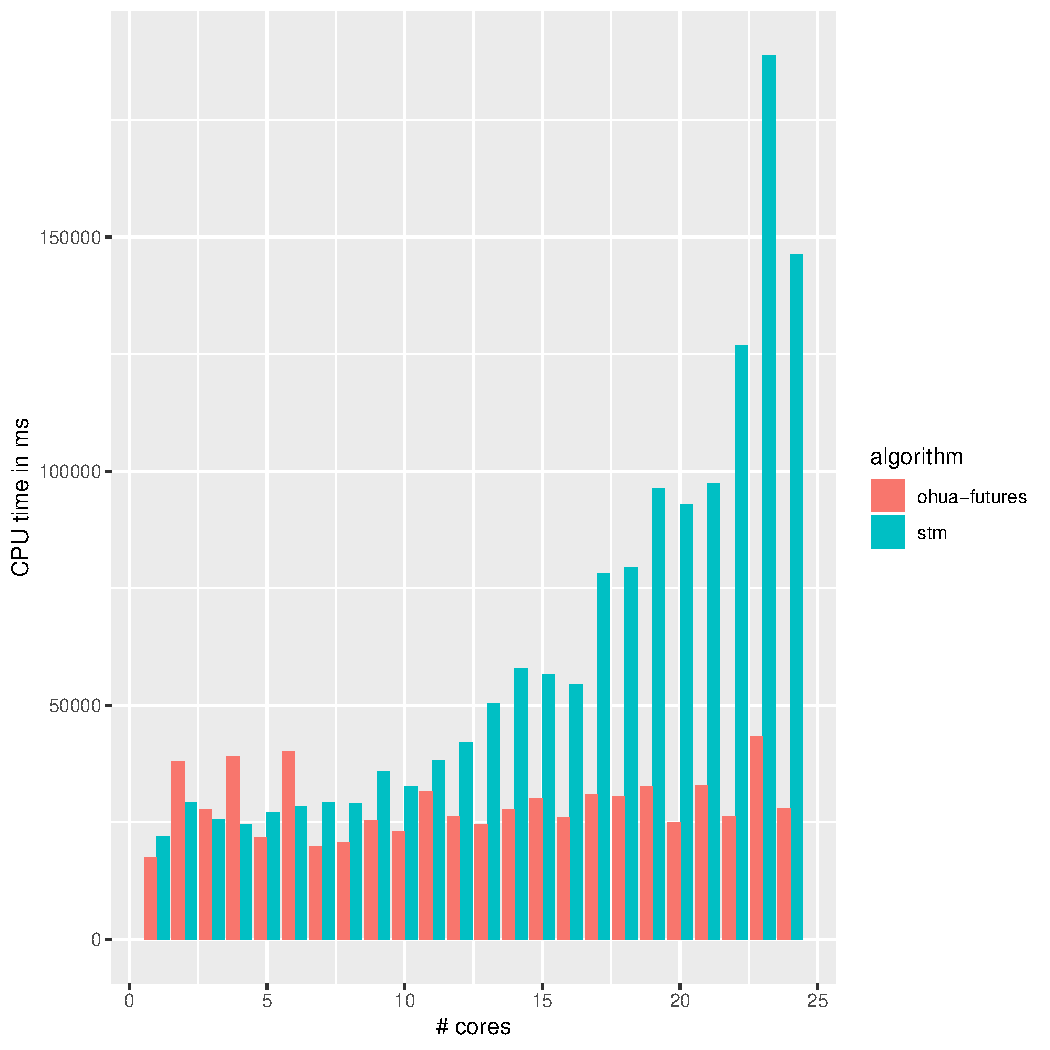
\includegraphics[width=\textwidth,keepaspectratio]{gfx/results/kmeans/kmeans-low++_cpu}
        %\caption{cpu usage kmeans-low++}%
    %\end{subfigure}%
    %\caption{Results of the kmeans-low benchmark.}%
    %\label{fig:evaulation:kmeans-low}
%\end{figure}

% - present benchmark results -- maybe for the manual Ohua implementation as well, if results differ
% - discuss why we perform better/worse at certain points
% - we see the determinism!
% - discuss energy usage etc
